\documentclass{article}  % Define la clase del documento.

% Paquetes de idioma y codificación
\usepackage[utf8]{inputenc}
\usepackage[T1]{fontenc}
%\usepackage[spanish]{babel}  % Ajusta el idioma del documento a español.
\usepackage{tabularx}  % Permite la creación de tablas con ancho ajustable.

\usepackage{caption}
\usepackage{subcaption}

% Paquete de geometría para configurar márgenes y tamaño de papel
\usepackage[letterpaper, margin=3cm]{geometry}

\usepackage[english]{babel}
\addto\captionsspanish{%
  \renewcommand{\tablename}{Table}%
  \renewcommand{\figurename}{Figure}%
}

% Paquetes de tipografía
\usepackage{mathptmx}    % Usa Times New Roman como fuente.
\usepackage{microtype}   % Mejora la justificación del texto.

% Paquetes para manejo de colores y gráficos
\usepackage{xcolor}      % Define y utiliza colores.
\usepackage{graphicx}    % Permite la inserción de imágenes.
\usepackage{tikz}        % Creación de gráficos vectoriales.

% Configuración de enlaces y referencias cruzadas
\usepackage{hyperref}
\hypersetup{
    colorlinks   = true,
    linkcolor    = darkblue,
    citecolor    = black,
    filecolor    = blue,
    urlcolor     = blue
}

\usepackage{media9} % Permite la inserción de multimedia.

% Paquetes para la mejora visual de tablas y figuras
\usepackage{booktabs}    % Para tablas de alta calidad.
\usepackage{float}       % Controla la posición de figuras y tablas.

% Paquete para la personalización de códigos fuente
\usepackage{listings}
\lstset{
    literate=
    {á}{{\'a}}1 {é}{{\'e}}1 {í}{{\'i}}1 {ó}{{\'o}}1 {ú}{{\'u}}1
    {Á}{{\'A}}1 {É}{{\'E}}1 {Í}{{\'I}}1 {Ó}{{\'O}}1 {Ú}{{\'U}}1
    {ñ}{{\~n}}1 {Ñ}{{\~N}}1 {ü}{{\"u}}1 {Ü}{{\"U}}1,
    backgroundcolor=\color{backcolour},
    commentstyle=\color{codegreen},
    keywordstyle=\color{codepurple},
    numberstyle=\tiny\color{codegray},
    stringstyle=\color{red},
    basicstyle=\ttfamily\small,
    breakatwhitespace=false,
    breaklines=true,
    captionpos=b,
    keepspaces=true,
    numbers=left,
    numbersep=5pt,
    showspaces=false,
    showstringspaces=false,
    showtabs=false,
    tabsize=2,
    language=TeX,
    morecomment=[l]\#,
    frame=single,
    rulecolor=\color{black}
}

% Definición de colores al estilo Visual Studio Code
\definecolor{darkblue}{rgb}{0.0, 0.0, 0.55}  % Enlaces
\definecolor{codegreen}{rgb}{0.25, 0.49, 0.48}  % Comentarios
\definecolor{codegray}{rgb}{0.5, 0.5, 0.5}  % Números y anotaciones
\definecolor{codepurple}{rgb}{0.58, 0, 0.82}  % Palabras clave
\definecolor{backcolour}{rgb}{0.95, 0.95, 0.92}  % Fondo de código

% Configuraciones de párrafo y matemáticas
\usepackage{amsmath}
\usepackage{parskip}    % Espaciado entre párrafos.
\usepackage{ragged2e}   % Justificación mejorada.
\usepackage{multicol}

% Configuración de secciones y encabezados
\usepackage{titlesec}
\titleclass{\part}{top} % Make part like a class
\titleformat{\part}[display]
  {\normalfont\huge\bfseries\centering}{\thepart}{40pt}{\Huge}
\titlespacing*{\part}{0pt}{-60pt}{10pt}
\titleformat{\part}
  {\normalfont\huge\bfseries}{}{0pt}{}

% Asegúrate de usar esto para mantener el estilo en las páginas de las partes
\titleformat{\part}[display]
  {\normalfont\huge\bfseries}{}{0pt}{}
  [\thispagestyle{fancy}] % Aplica el estilo fancy a las páginas de las partes

% Configuración de encabezados y pies de página personalizados
\usepackage{fancyhdr}
\pagestyle{fancy}
\fancyhf{}
\fancyhead[L]{\raisebox{0.20cm}{\textbf{Dynamics of structures}}}
\fancyhead[R]{\raisebox{0.1cm}{
\includegraphics[width=0.25\linewidth]{img/LOGO_UNIVERSIDAD.jpg}}}
\fancyhead[C]{\rule{\textwidth}{0.6pt}}
\fancyfoot[C]{\rule{\textwidth}{0.6pt}}
\fancyfoot[R]{\raisebox{-1.5\baselineskip}{\thepage}}
\renewcommand{\headrulewidth}{0pt}
\renewcommand{\footrulewidth}{0pt}

% Configuración avanzada de geometría
\geometry{
  top=3.5cm, % Aumenta el espacio en la parte superior para subir el encabezado
  bottom=2.5cm,
  headheight=2.5cm % Aumenta la altura del encabezado si es necesario
}

% Configuracion de bibliografia
\usepackage{natbib}
\bibliographystyle{unsrtnat}  % Puedes cambiarlo por `unsrtnat`, `abbrvnat`, etc.

\begin{document}
%----------------------------------------------------------------------------------------
% PORTADA
%----------------------------------------------------------------------------------------
\begin{titlepage}%Inicio de la carátula, solo modificar los datos necesarios
\newcommand{\HRule}{\rule{\linewidth}{0.5mm}} 
\center 
%----------------------------------------------------------------------------------------
%	ENCABEZADO
%----------------------------------------------------------------------------------------

\includegraphics[width=10cm]{img/LOGO_UNIVERSIDAD.jpg}\\ % Si esta plantilla se copio correctamente, va a llevar la imagen del logo de la facultad.OBS: Es necesario incluir el paquete: graphicx
\vspace{3cm}
%----------------------------------------------------------------------------------------
%	SECCION DEL TITULO
%----------------------------------------------------------------------------------------
\HRule \\[0.4cm]
{ \huge \bfseries Finite Elements}\\[0.4cm] % Titulo del documento
{ \huge \bfseries Homework N°3 - Final Report}\\[0.4cm] % Titulo del documento
\HRule \\[1.5cm]
 \vspace{5cm}
%----------------------------------------------------------------------------------------
%	SECCION DEL AUTOR
%----------------------------------------------------------------------------------------
\begin{flushright}
  { \textbf{Professor:}\\
  Jose Antonio Abell\\
  \textbf{Assistance:}\\
  Nicolás Mora\\
  \textbf{Students:} \\
  Felipe Vicencio\\
  Lukas Wolff\\
}
\end{flushright}
\vspace{1cm}
%----------------------------------------------------------------------------------------
%	SECCION DE LA FECHA
%----------------------------------------------------------------------------------------
{\large \textbf{\today}}\\[2cm] % El comando \today coloca la fecha del dia, y esto se actualiza con cada compilacion, en caso de querer tener una fecha estatica, reemplazar el \today por la fecha deseada
\end{titlepage}

\newpage
\thispagestyle{empty} % Deshabilita el número de página en la página del índice

%----------------------------------------------------------------------------------------
%  INDICE
%----------------------------------------------------------------------------------------
%\newpage
%\thispagestyle{empty} % Deshabilita el número de página en la página del índice
%\tableofcontents
%\thispagestyle{plain} % Deshabilita el encabezado en la página del índice
%\thispagestyle{empty} % Deshabilita el número de página en la página del índice
%\newpage

%\newpage
%\thispagestyle{empty}
%\listoffigures 
%\thispagestyle{plain} % Deshabilita el encabezado en la página del índice %
%\thispagestyle{empty}
\newpage
%----------------------------------------------------------------------------------------
%ACÁ EMPIEZA EL INFORME
\setcounter{page}{1}
%----------------------------------------------------------------------------------------
\section{Introduction}

Over the course of this excercise, we have deepend our understanding of three core aspects. Comprehending the Quad4 and Quad9 elements, implementing desing and analysis of structures on GMSH \textit{software} and optimizing the strcutures depending on its internal stresses and displacements.

\section{Results}

As the complete stucture to analize was symmetrical, only a half of it was modeled with a transfinite mesh and studied, as shown bellow.

\begin{figure}[H]
    \centering
    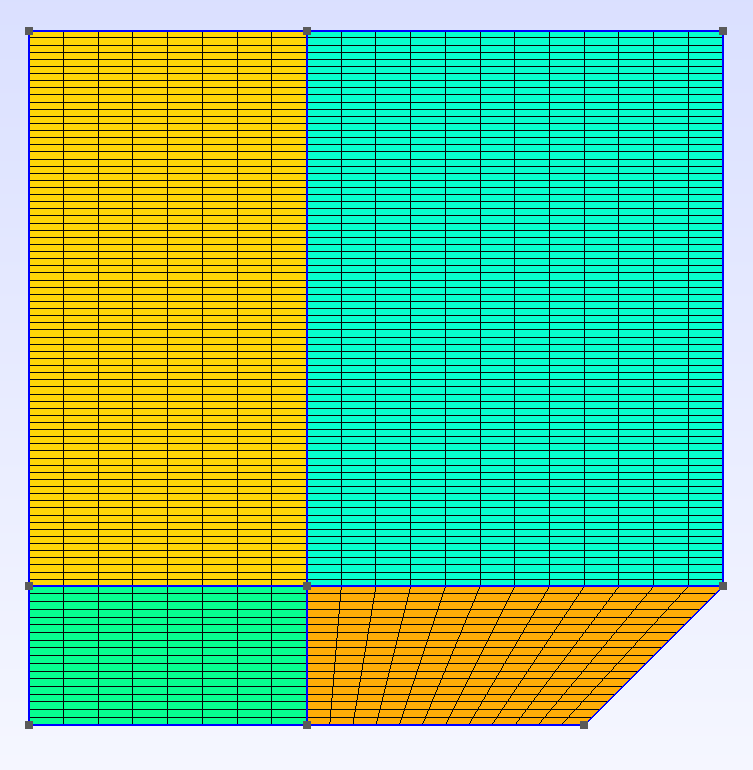
\includegraphics[width=0.5\textwidth]{img/geometria.png}
    \caption{Half structure modeled in GMSH}
    \label{fig:half_structure}
\end{figure}

\subsection{Part b) PONER LOS GRAFICOS LOCALES}

In this section, a stress analysis was made over 4 different mesh sizes using two refinment techniques, global and local refinment, for both element types.

For the global refinment, the characteristic size h was modified uniformly across the entire mesh, varying its value from 2 mm up to 1.25 mm. These values were determined based on the time required for the simulation to run and the capacity of the software to refine the mesh.

In the case of local refinment, the characteristic size h was modified in a specific region of the mesh, near the stress concentration area, in other words, the right border. For this to be studied, the number of elements was higher in that zone compared to the left border.

The results of refining the mesh globally and locally are shown in the following sections.

\subsubsection{Quad4 Element}

The following maps shows how the stress distribution changes with the mesh size as it is refined using Quad4 elements.

\begin{figure}[H]
  \centering
  \begin{subfigure}[b]{0.45\textwidth}
    \centering
    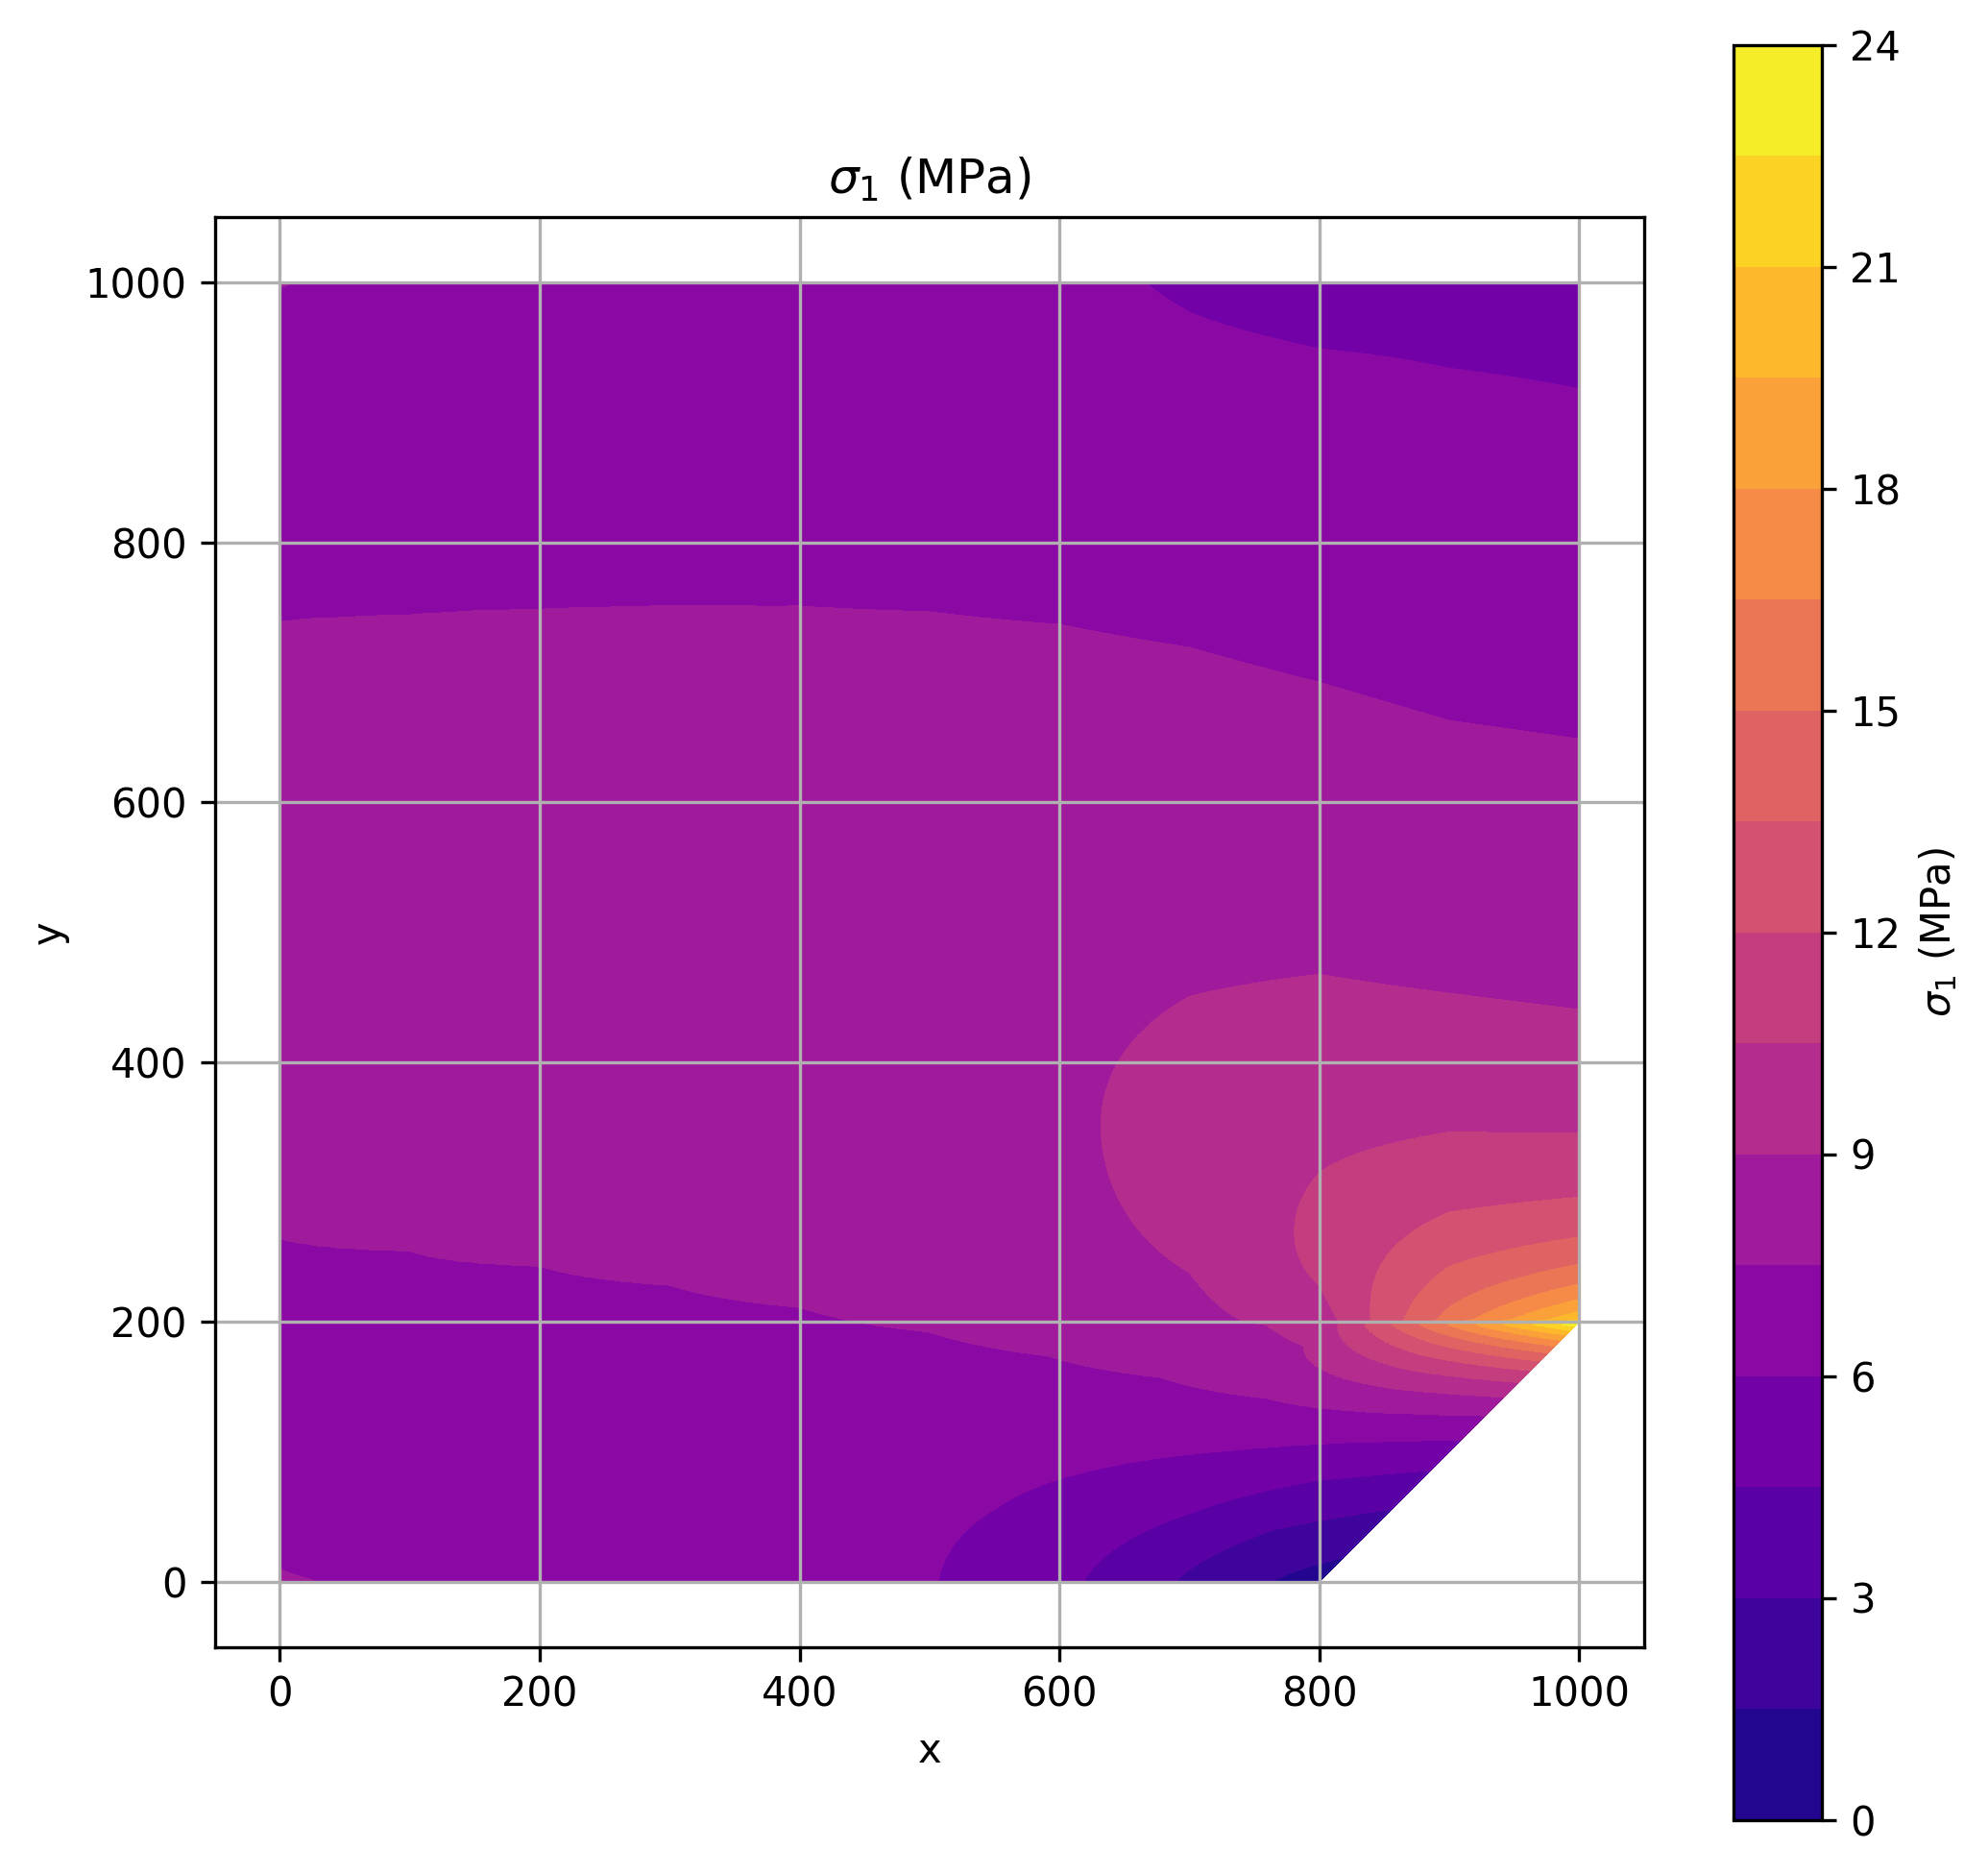
\includegraphics[width=\textwidth]{GRAFICOS/Quad4/2mm_global/resultados - sigma_1.png}
    \caption{Global mesh refinement - $h=2mm$}
    \label{fig:img1}
  \end{subfigure}
  \hfill
  \begin{subfigure}[b]{0.45\textwidth}
    \centering
    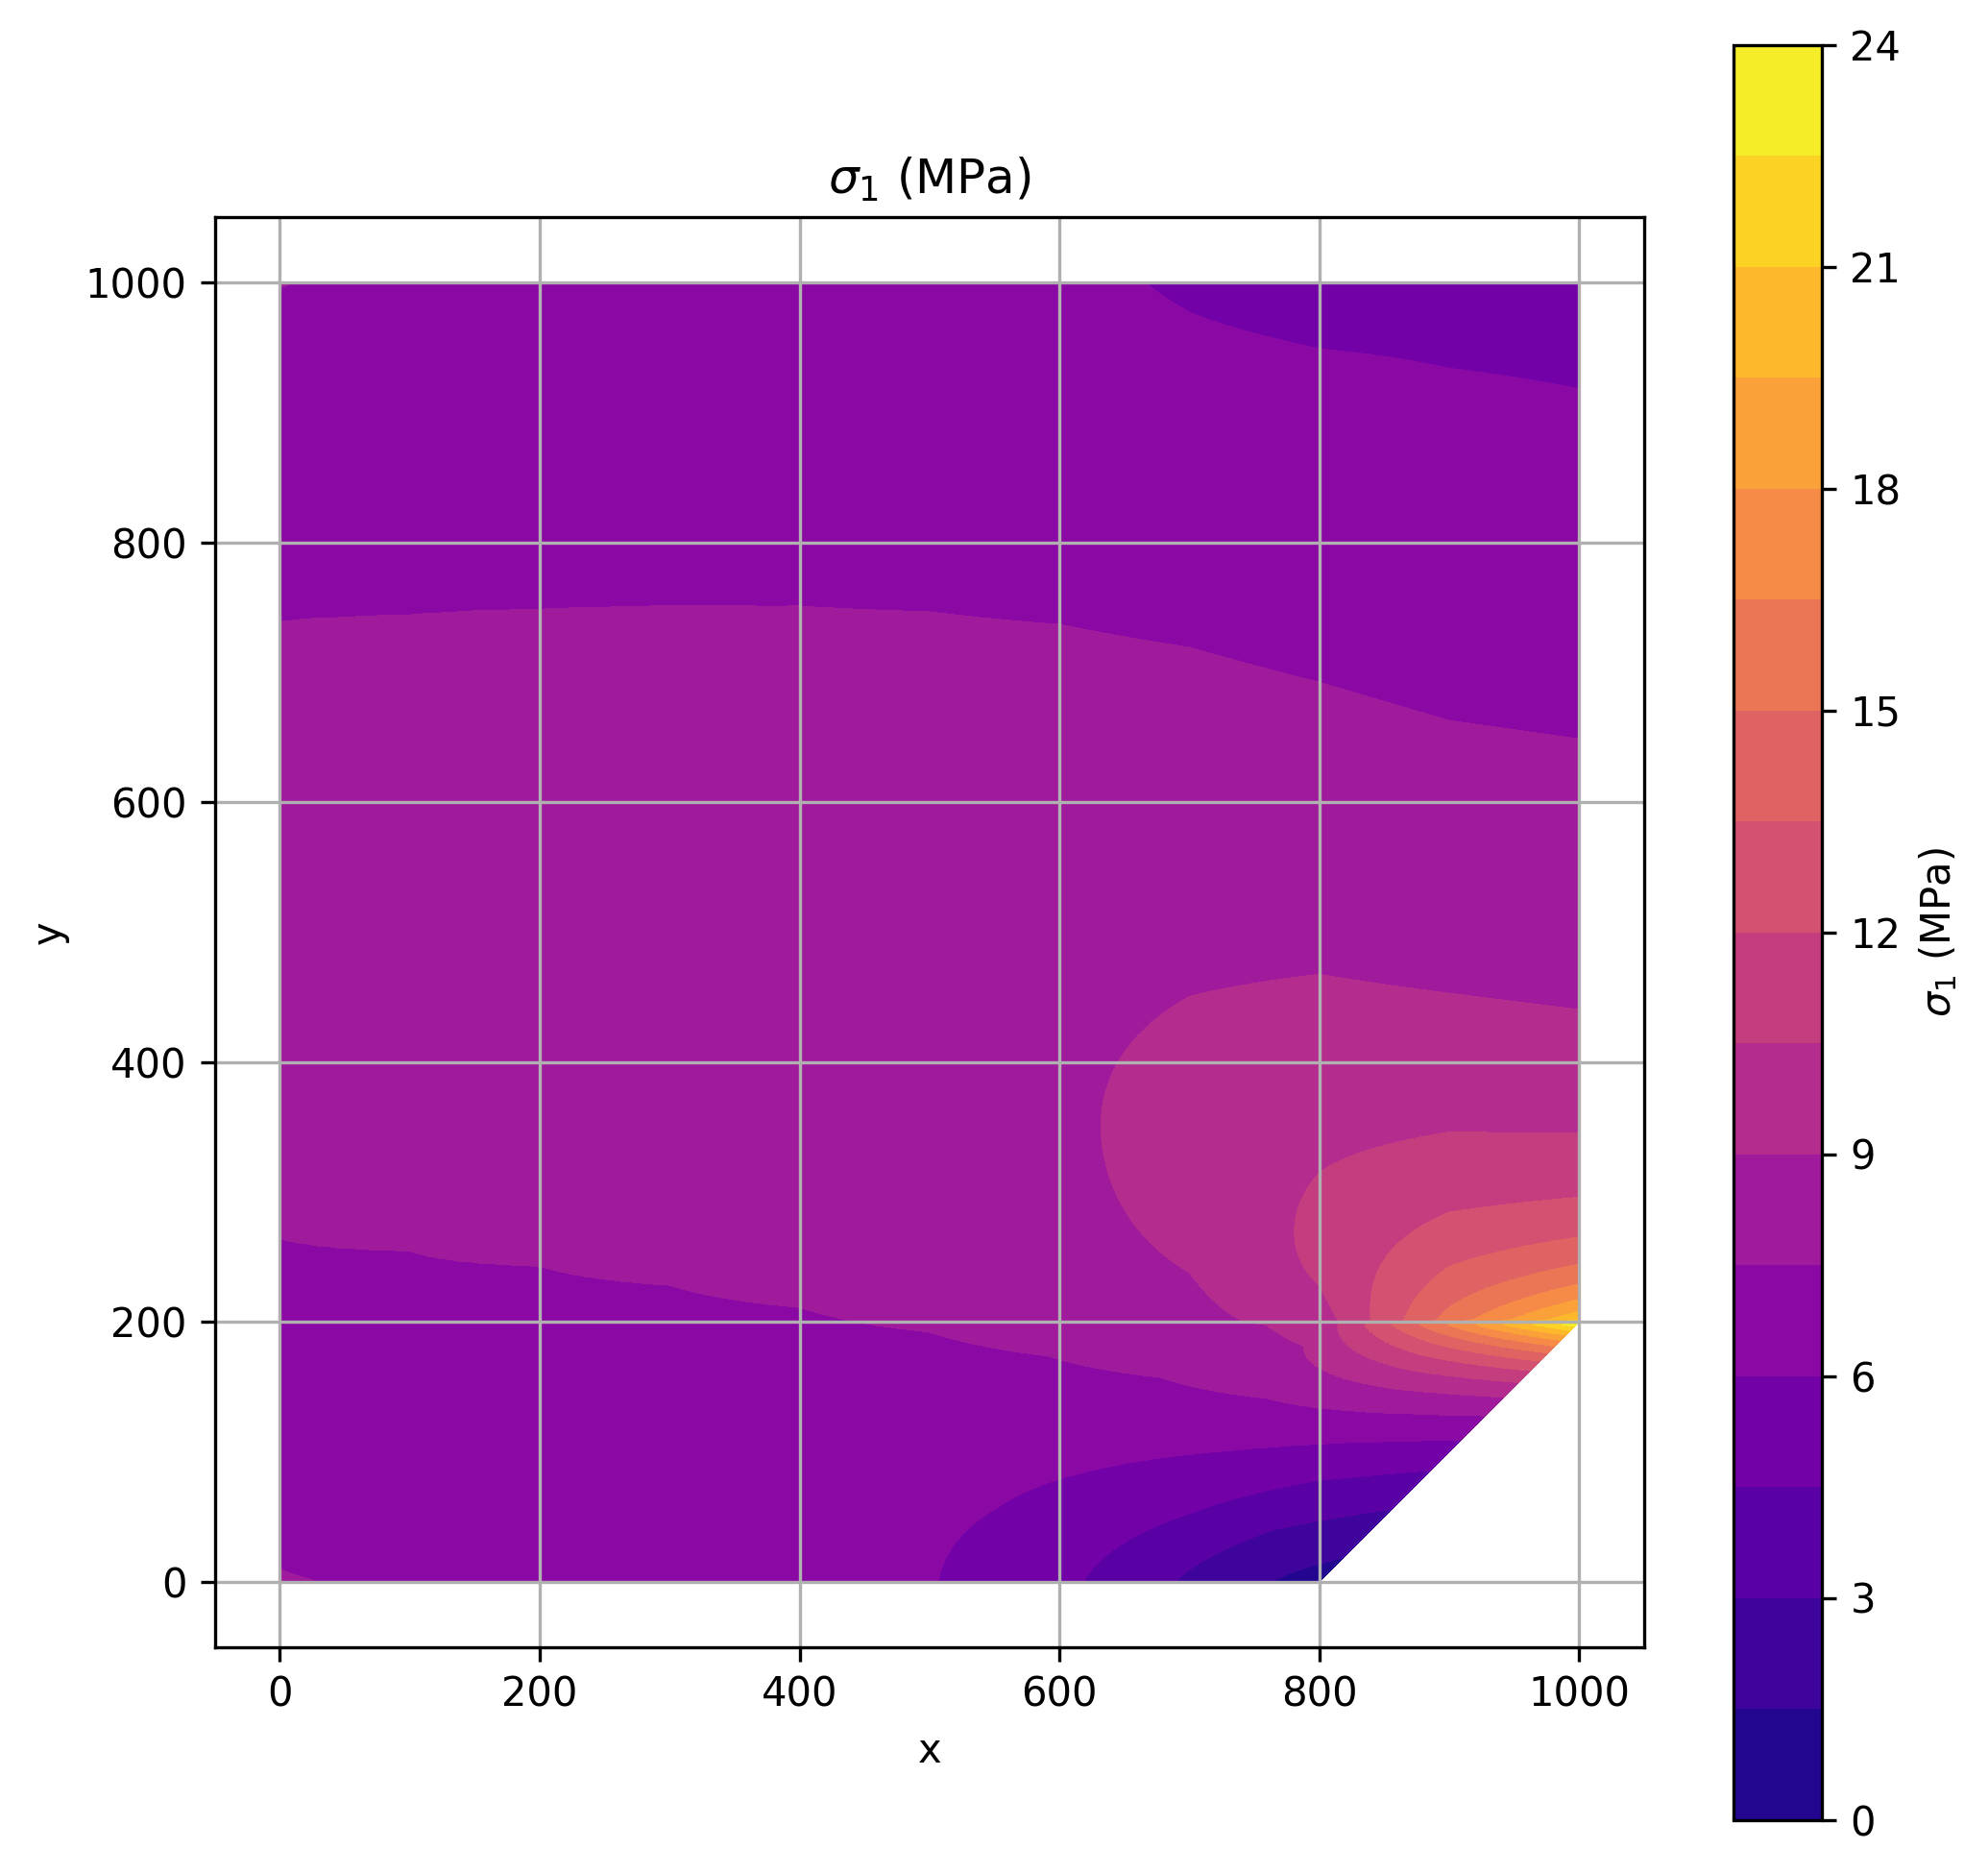
\includegraphics[width=\textwidth]{GRAFICOS/Quad4/2mm_global/resultados - sigma_1.png}
    \caption{Local mesh refinement - $h=2mm$}
    \label{fig:img2}
  \end{subfigure}
\end{figure}

\begin{figure}[H]
  \centering
  \begin{subfigure}[b]{0.45\textwidth}
    \centering
    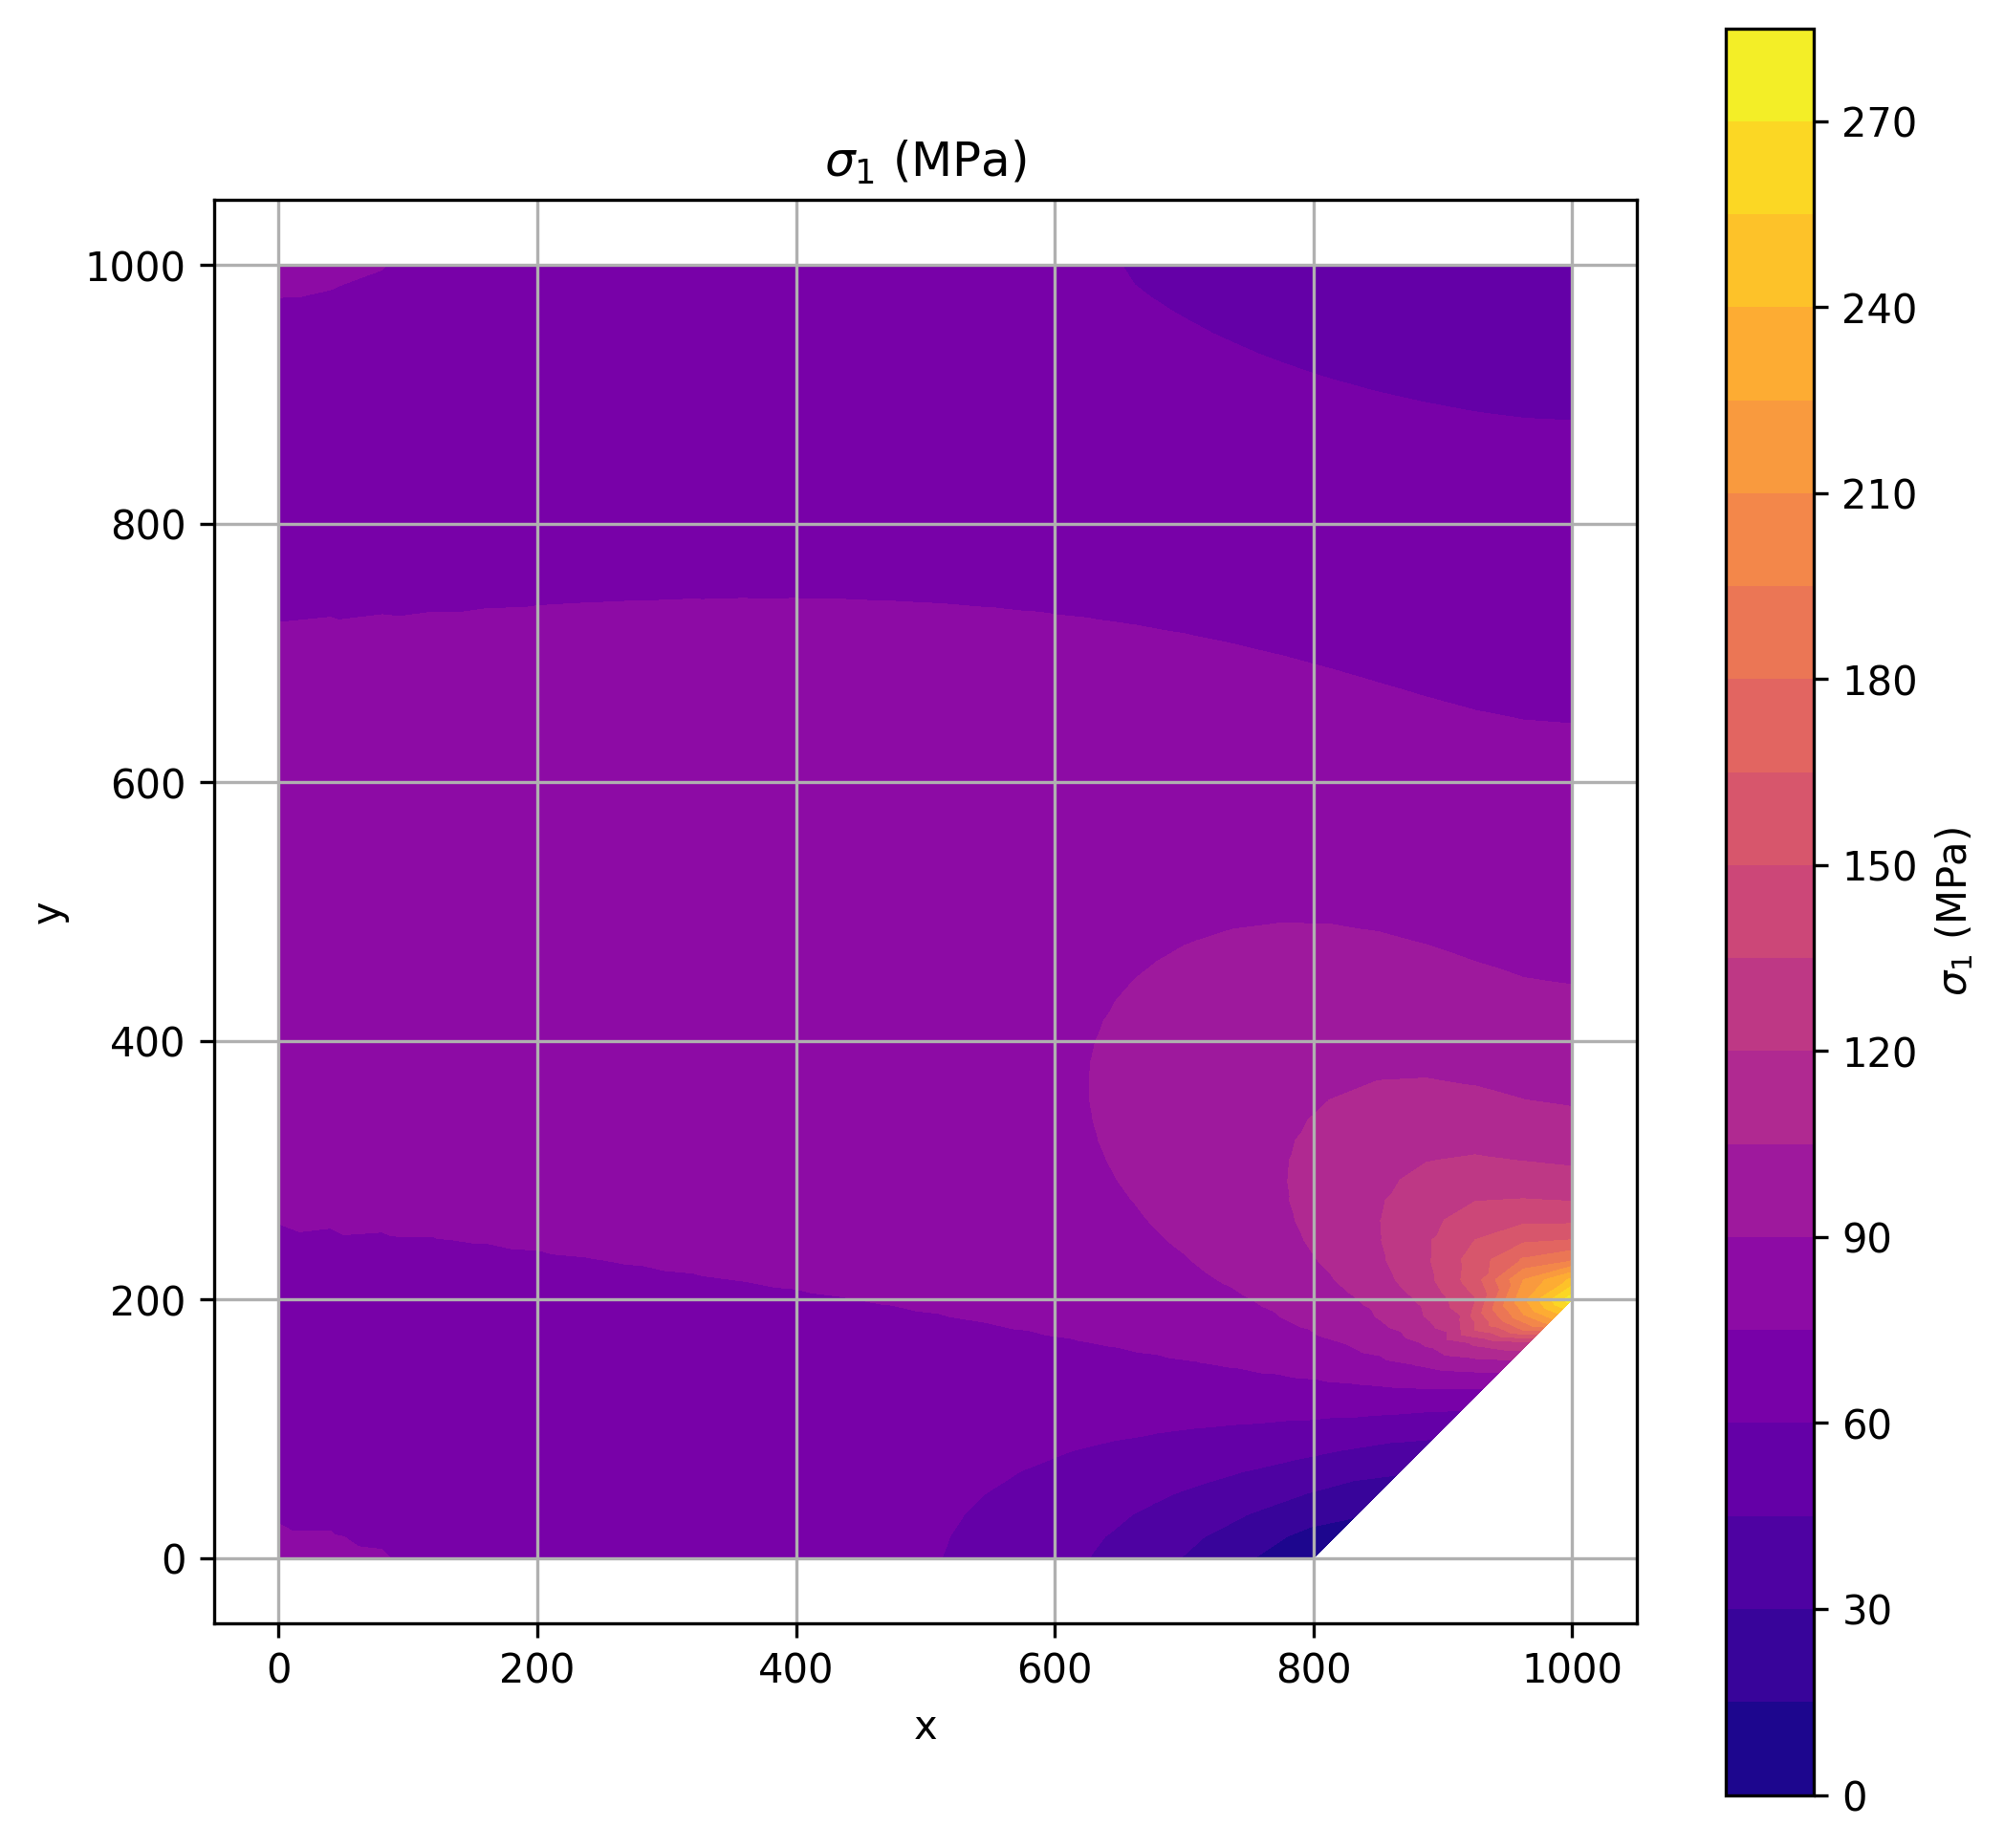
\includegraphics[width=\textwidth]{GRAFICOS/Quad4/1.75mm_global/resultados - sigma_1.png}
    \caption{Global mesh refinement - $h=1.75mm$}
    \label{fig:img11}
  \end{subfigure}
  \hfill
  \begin{subfigure}[b]{0.45\textwidth}
    \centering
    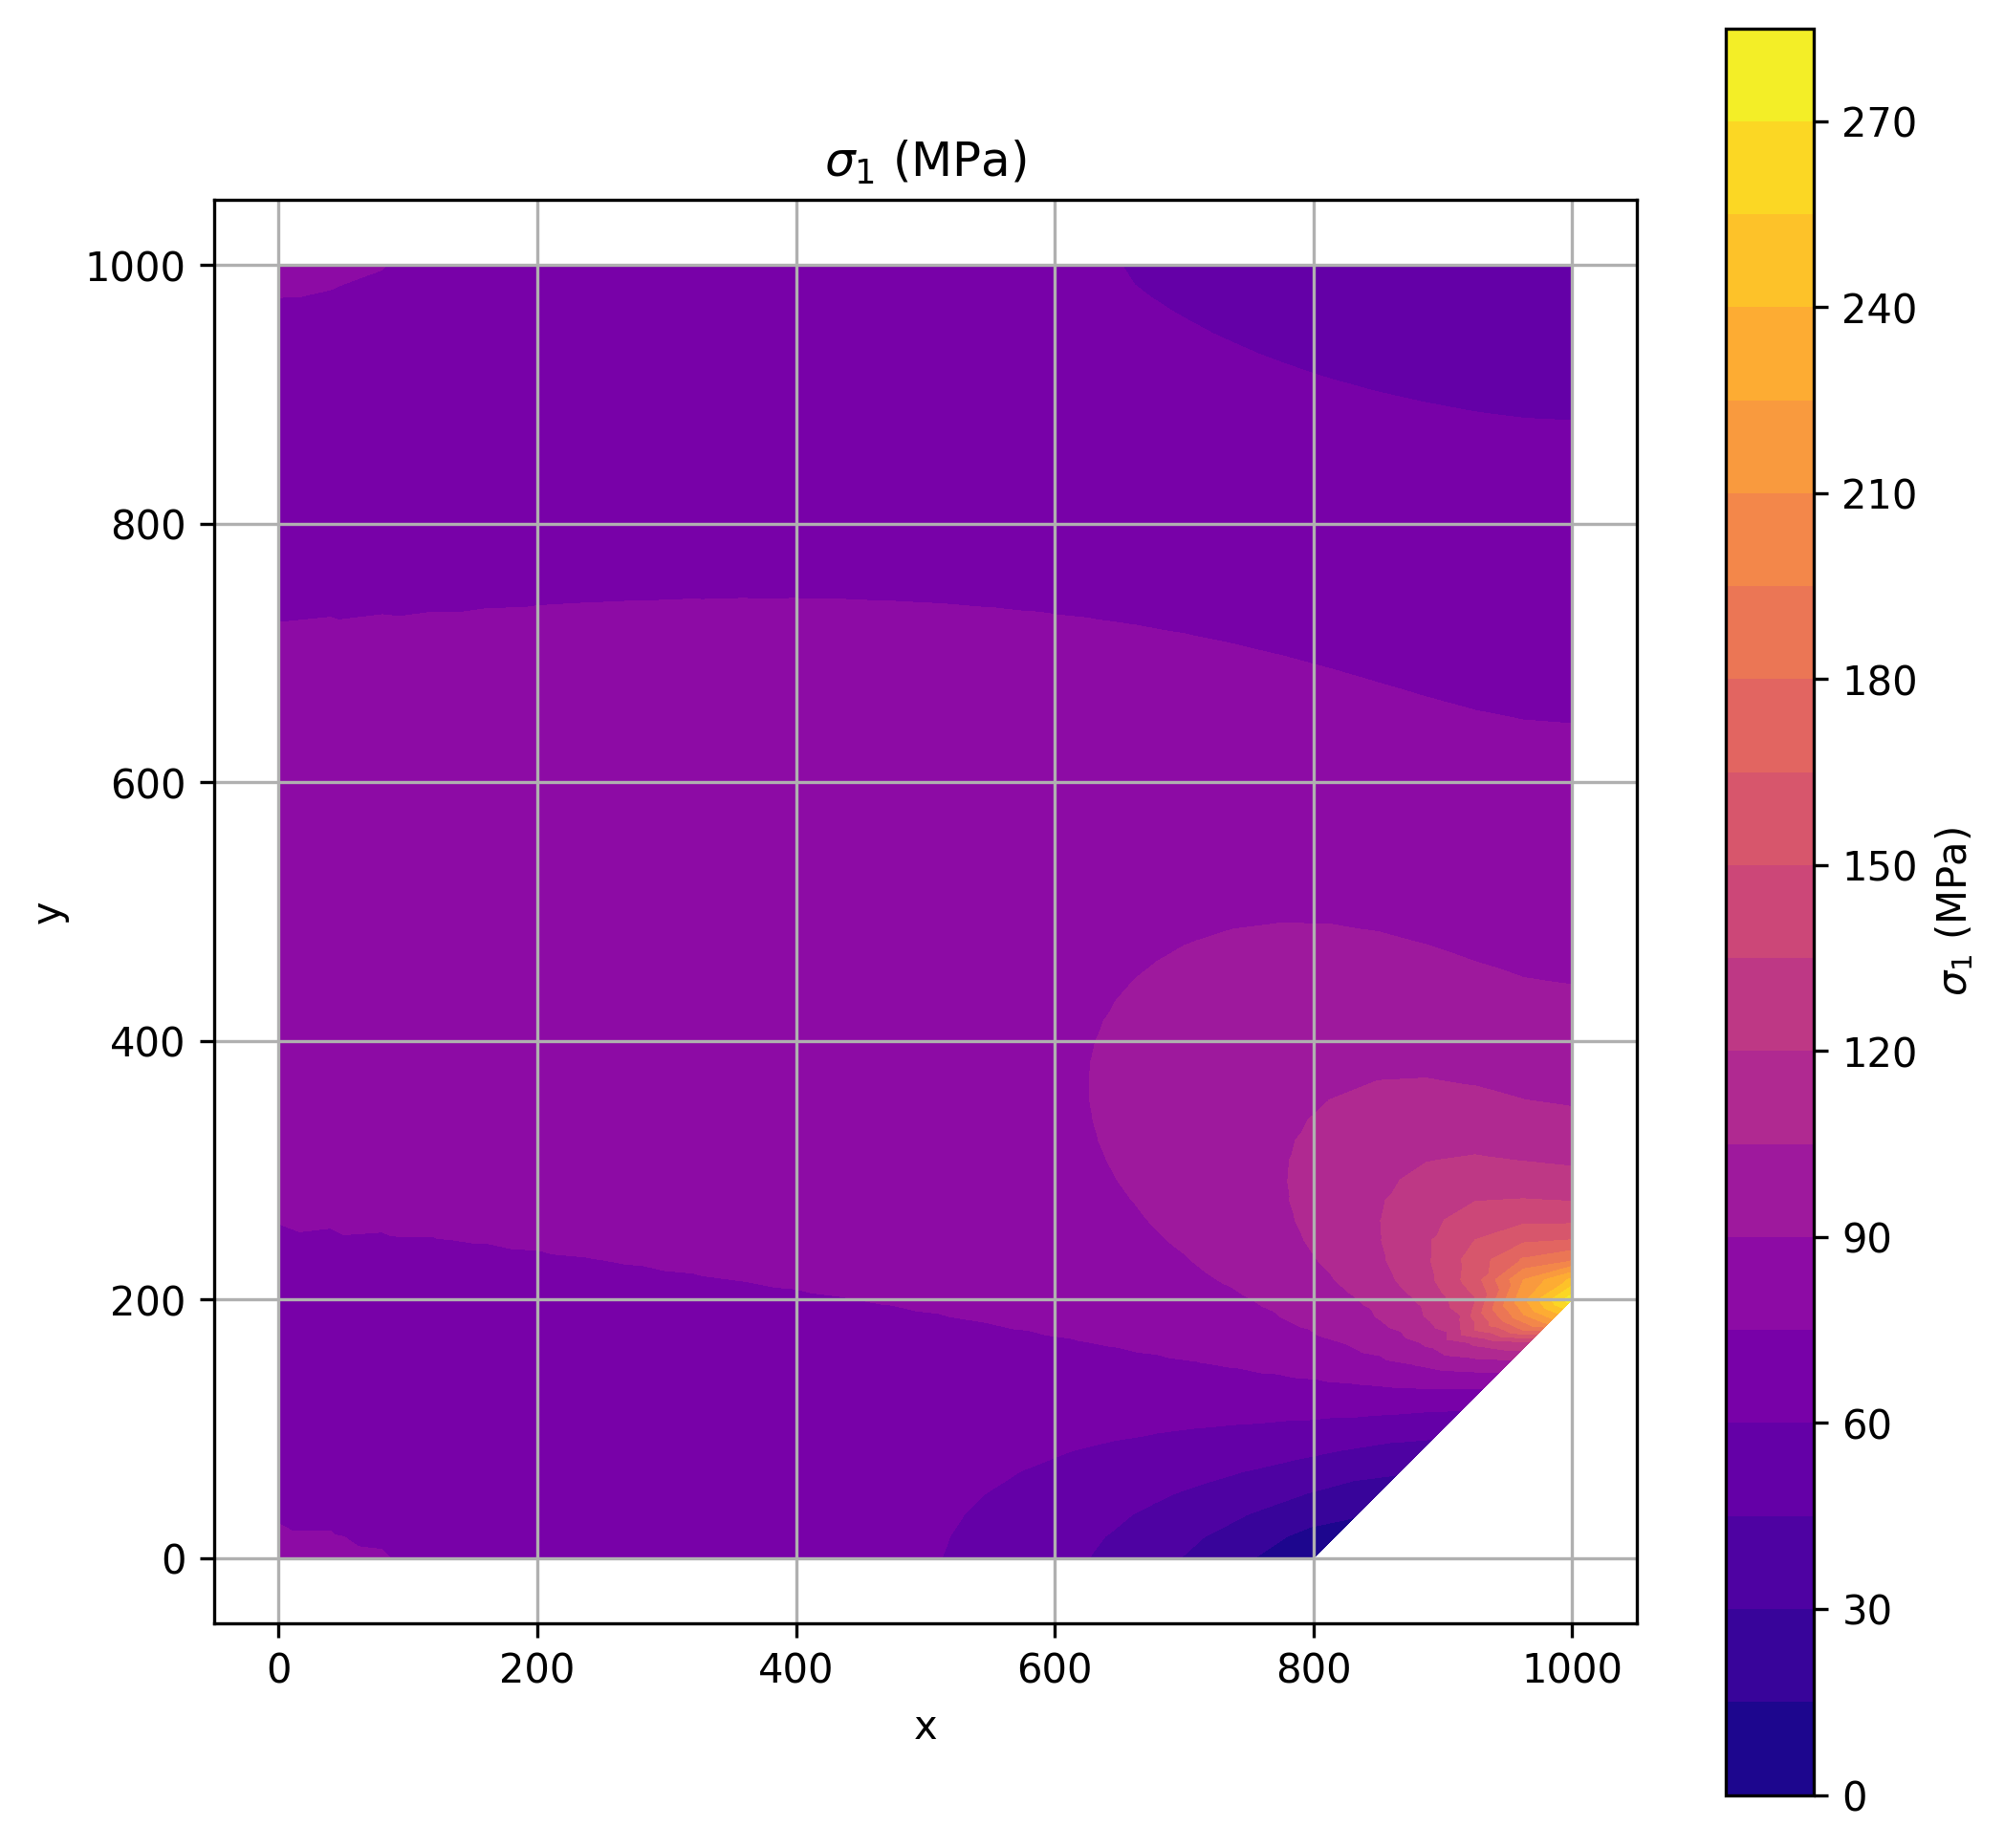
\includegraphics[width=\textwidth]{GRAFICOS/Quad4/1.75mm_global/resultados - sigma_1.png}
    \caption{Local mesh refinement - $h=1.75mm$}
    \label{fig:img21}
  \end{subfigure}
\end{figure}

\begin{figure}[H]
  \centering
  \begin{subfigure}[b]{0.45\textwidth}
    \centering
    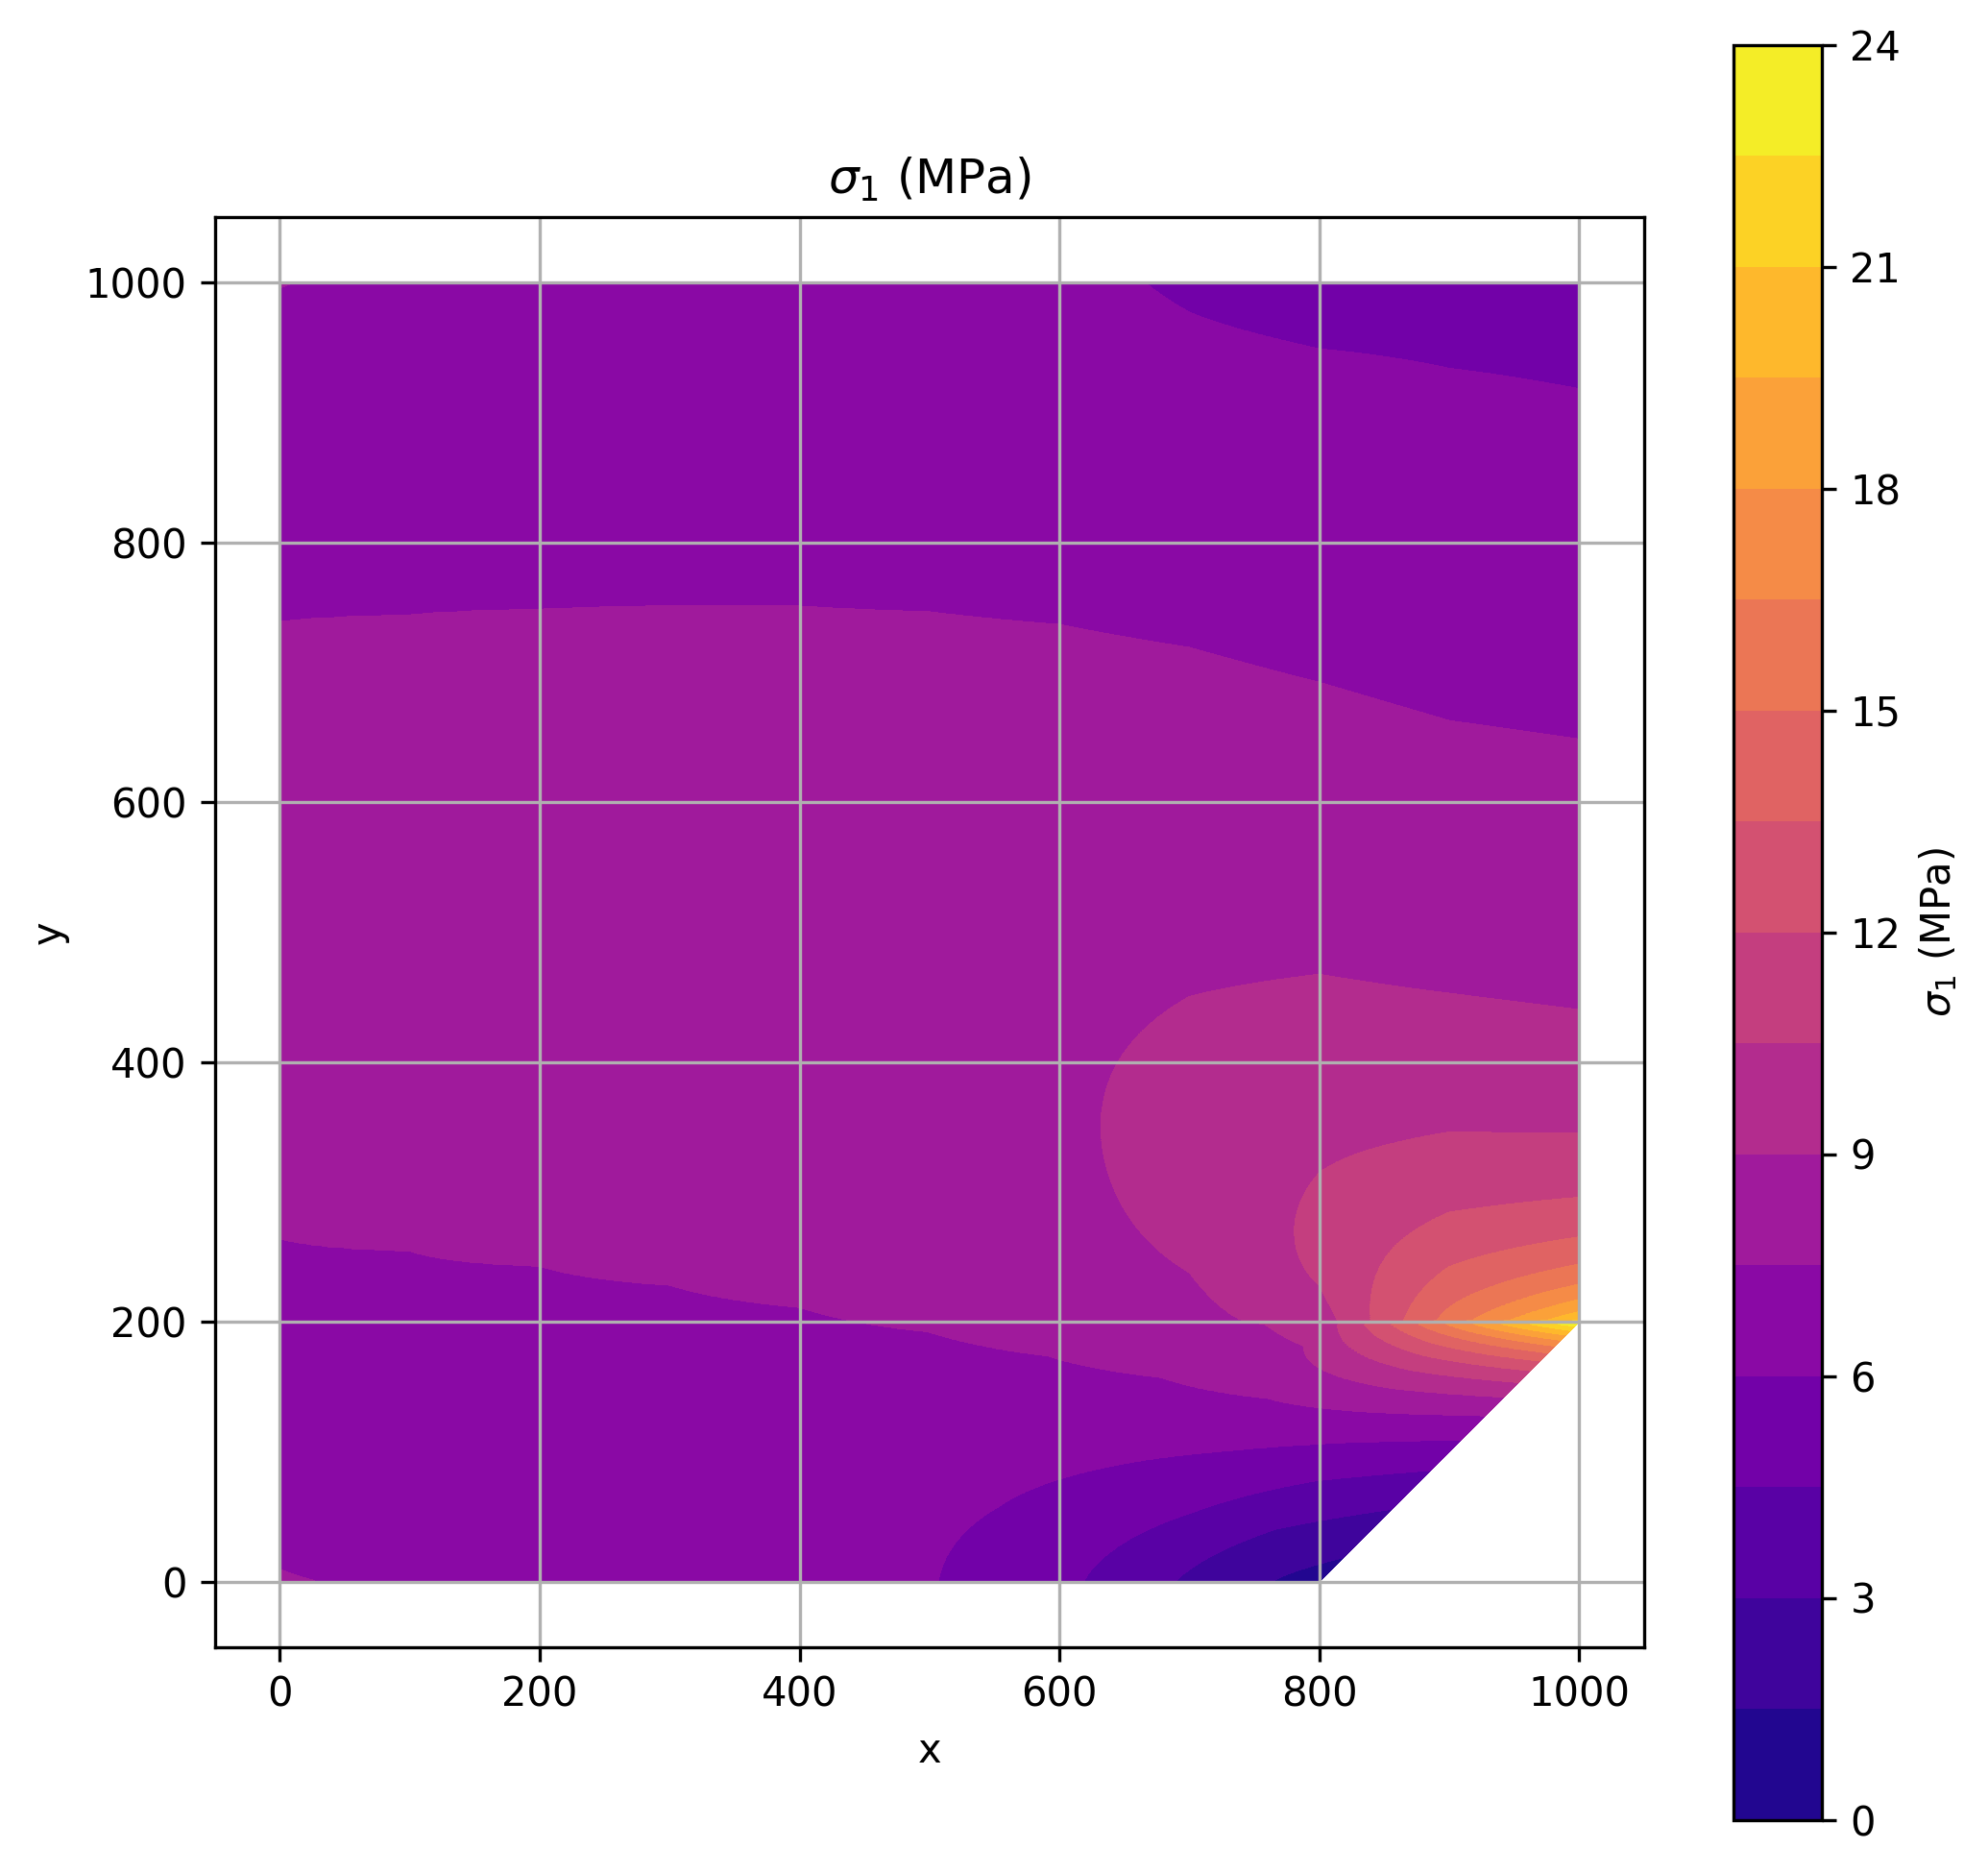
\includegraphics[width=\textwidth]{GRAFICOS/Quad4/1.5mm_global/resultados - sigma_1.png}
    \caption{Global mesh refinement - $h=1.5mm$}
    \label{fig:img12}
  \end{subfigure}
  \hfill
  \begin{subfigure}[b]{0.45\textwidth}
    \centering
    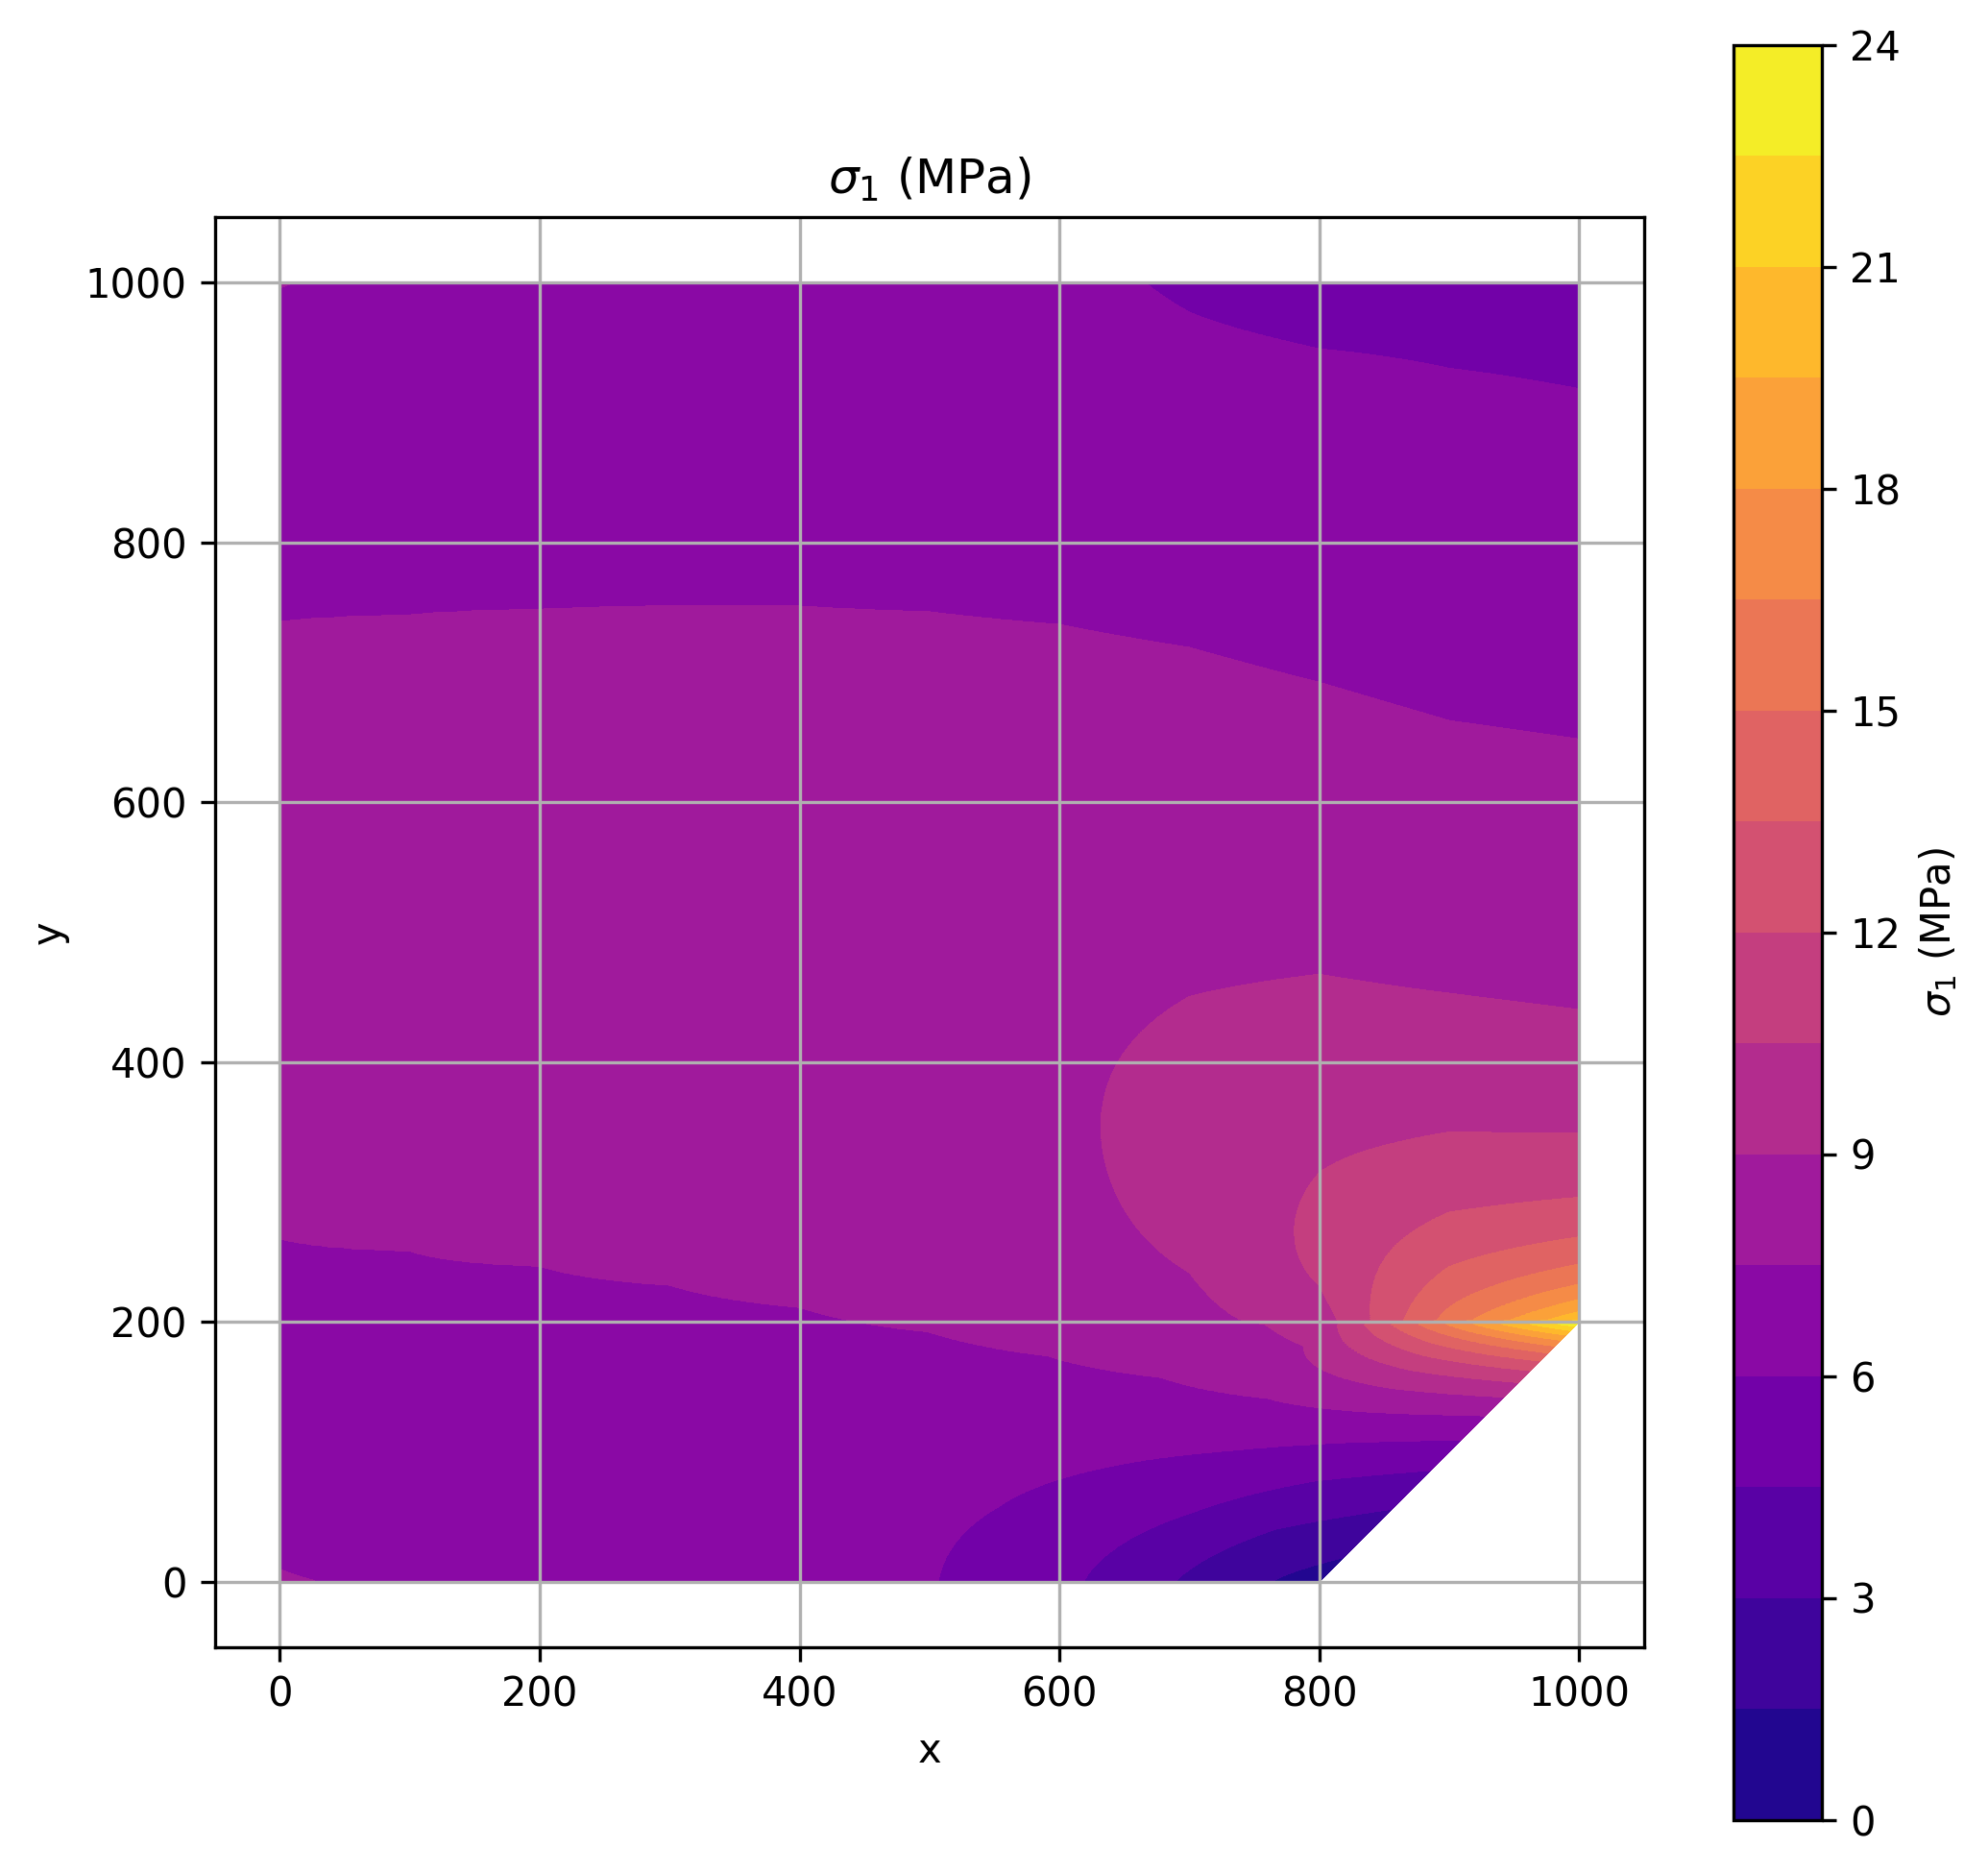
\includegraphics[width=\textwidth]{GRAFICOS/Quad4/1.5mm_global/resultados - sigma_1.png}
    \caption{Local mesh refinement - $h=1.5mm$}
    \label{fig:img22}
  \end{subfigure}
\end{figure}

\begin{figure}[H]
  \centering
  \begin{subfigure}[b]{0.45\textwidth}
    \centering
    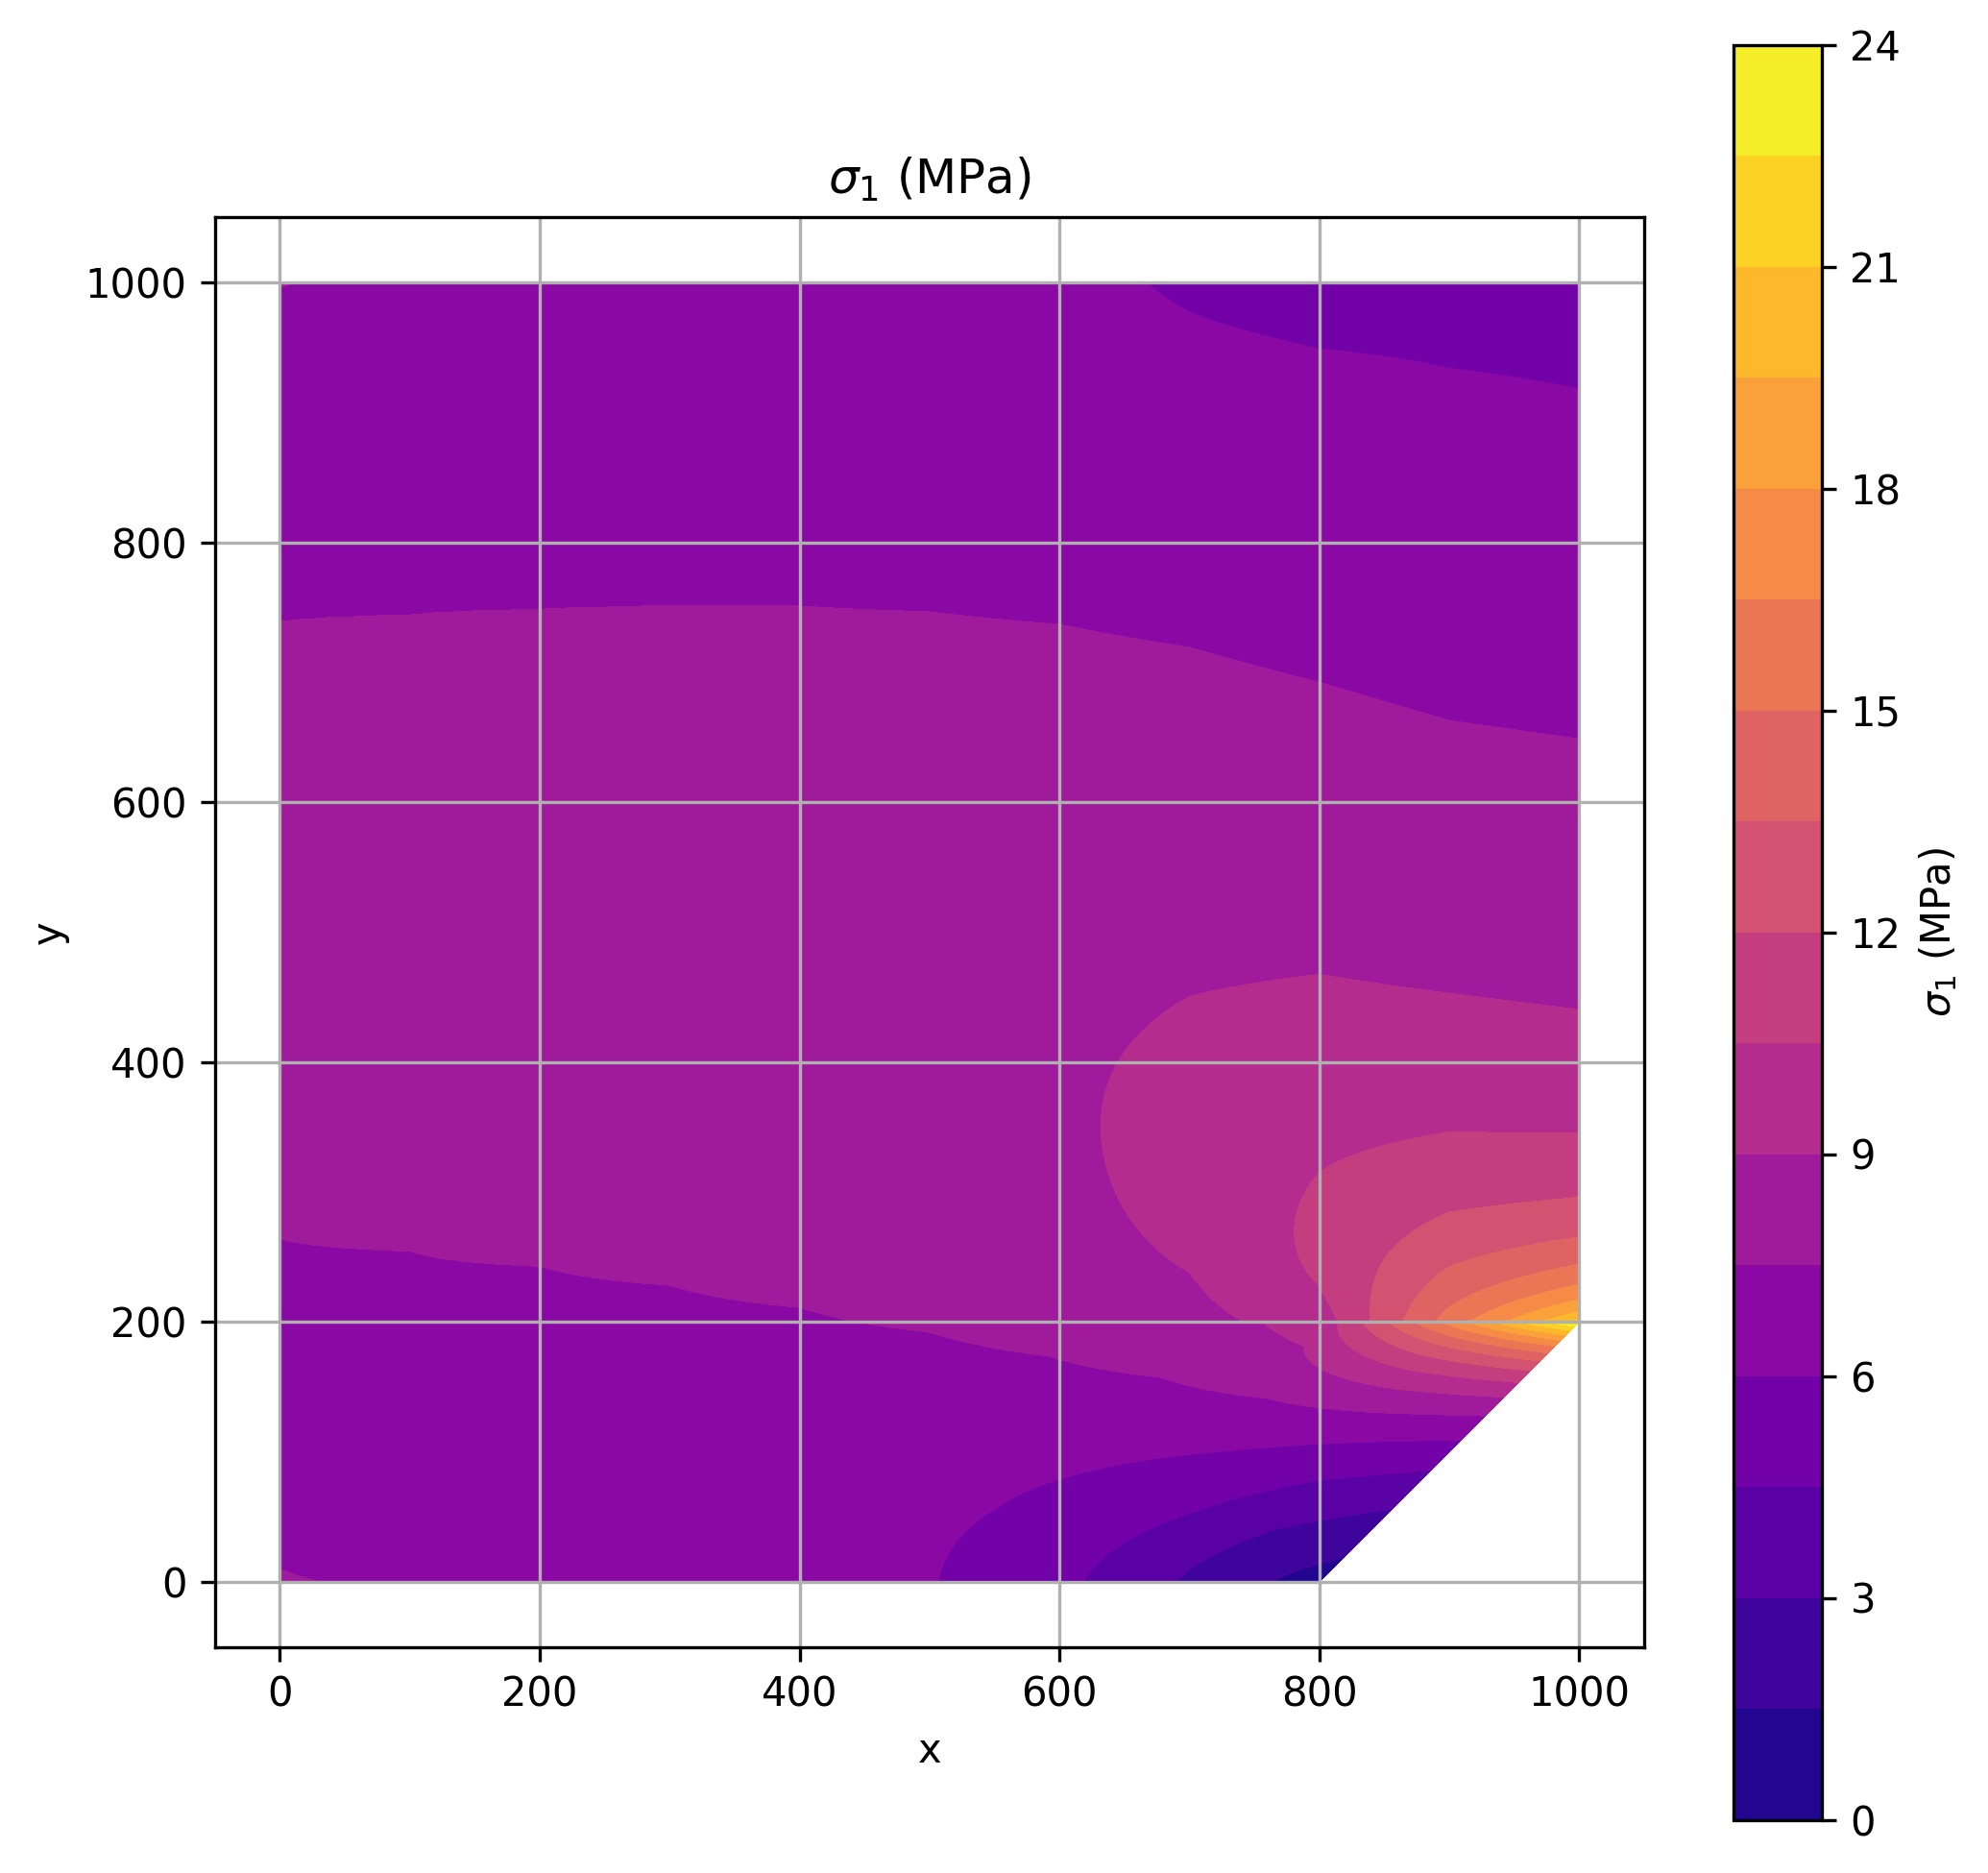
\includegraphics[width=\textwidth]{GRAFICOS/Quad4/1.25mm_global/resultados - sigma_1.png}
    \caption{Global mesh refinement - $h=1.25mm$}
    \label{fig:img13}
  \end{subfigure}
  \hfill
  \begin{subfigure}[b]{0.45\textwidth}
    \centering
    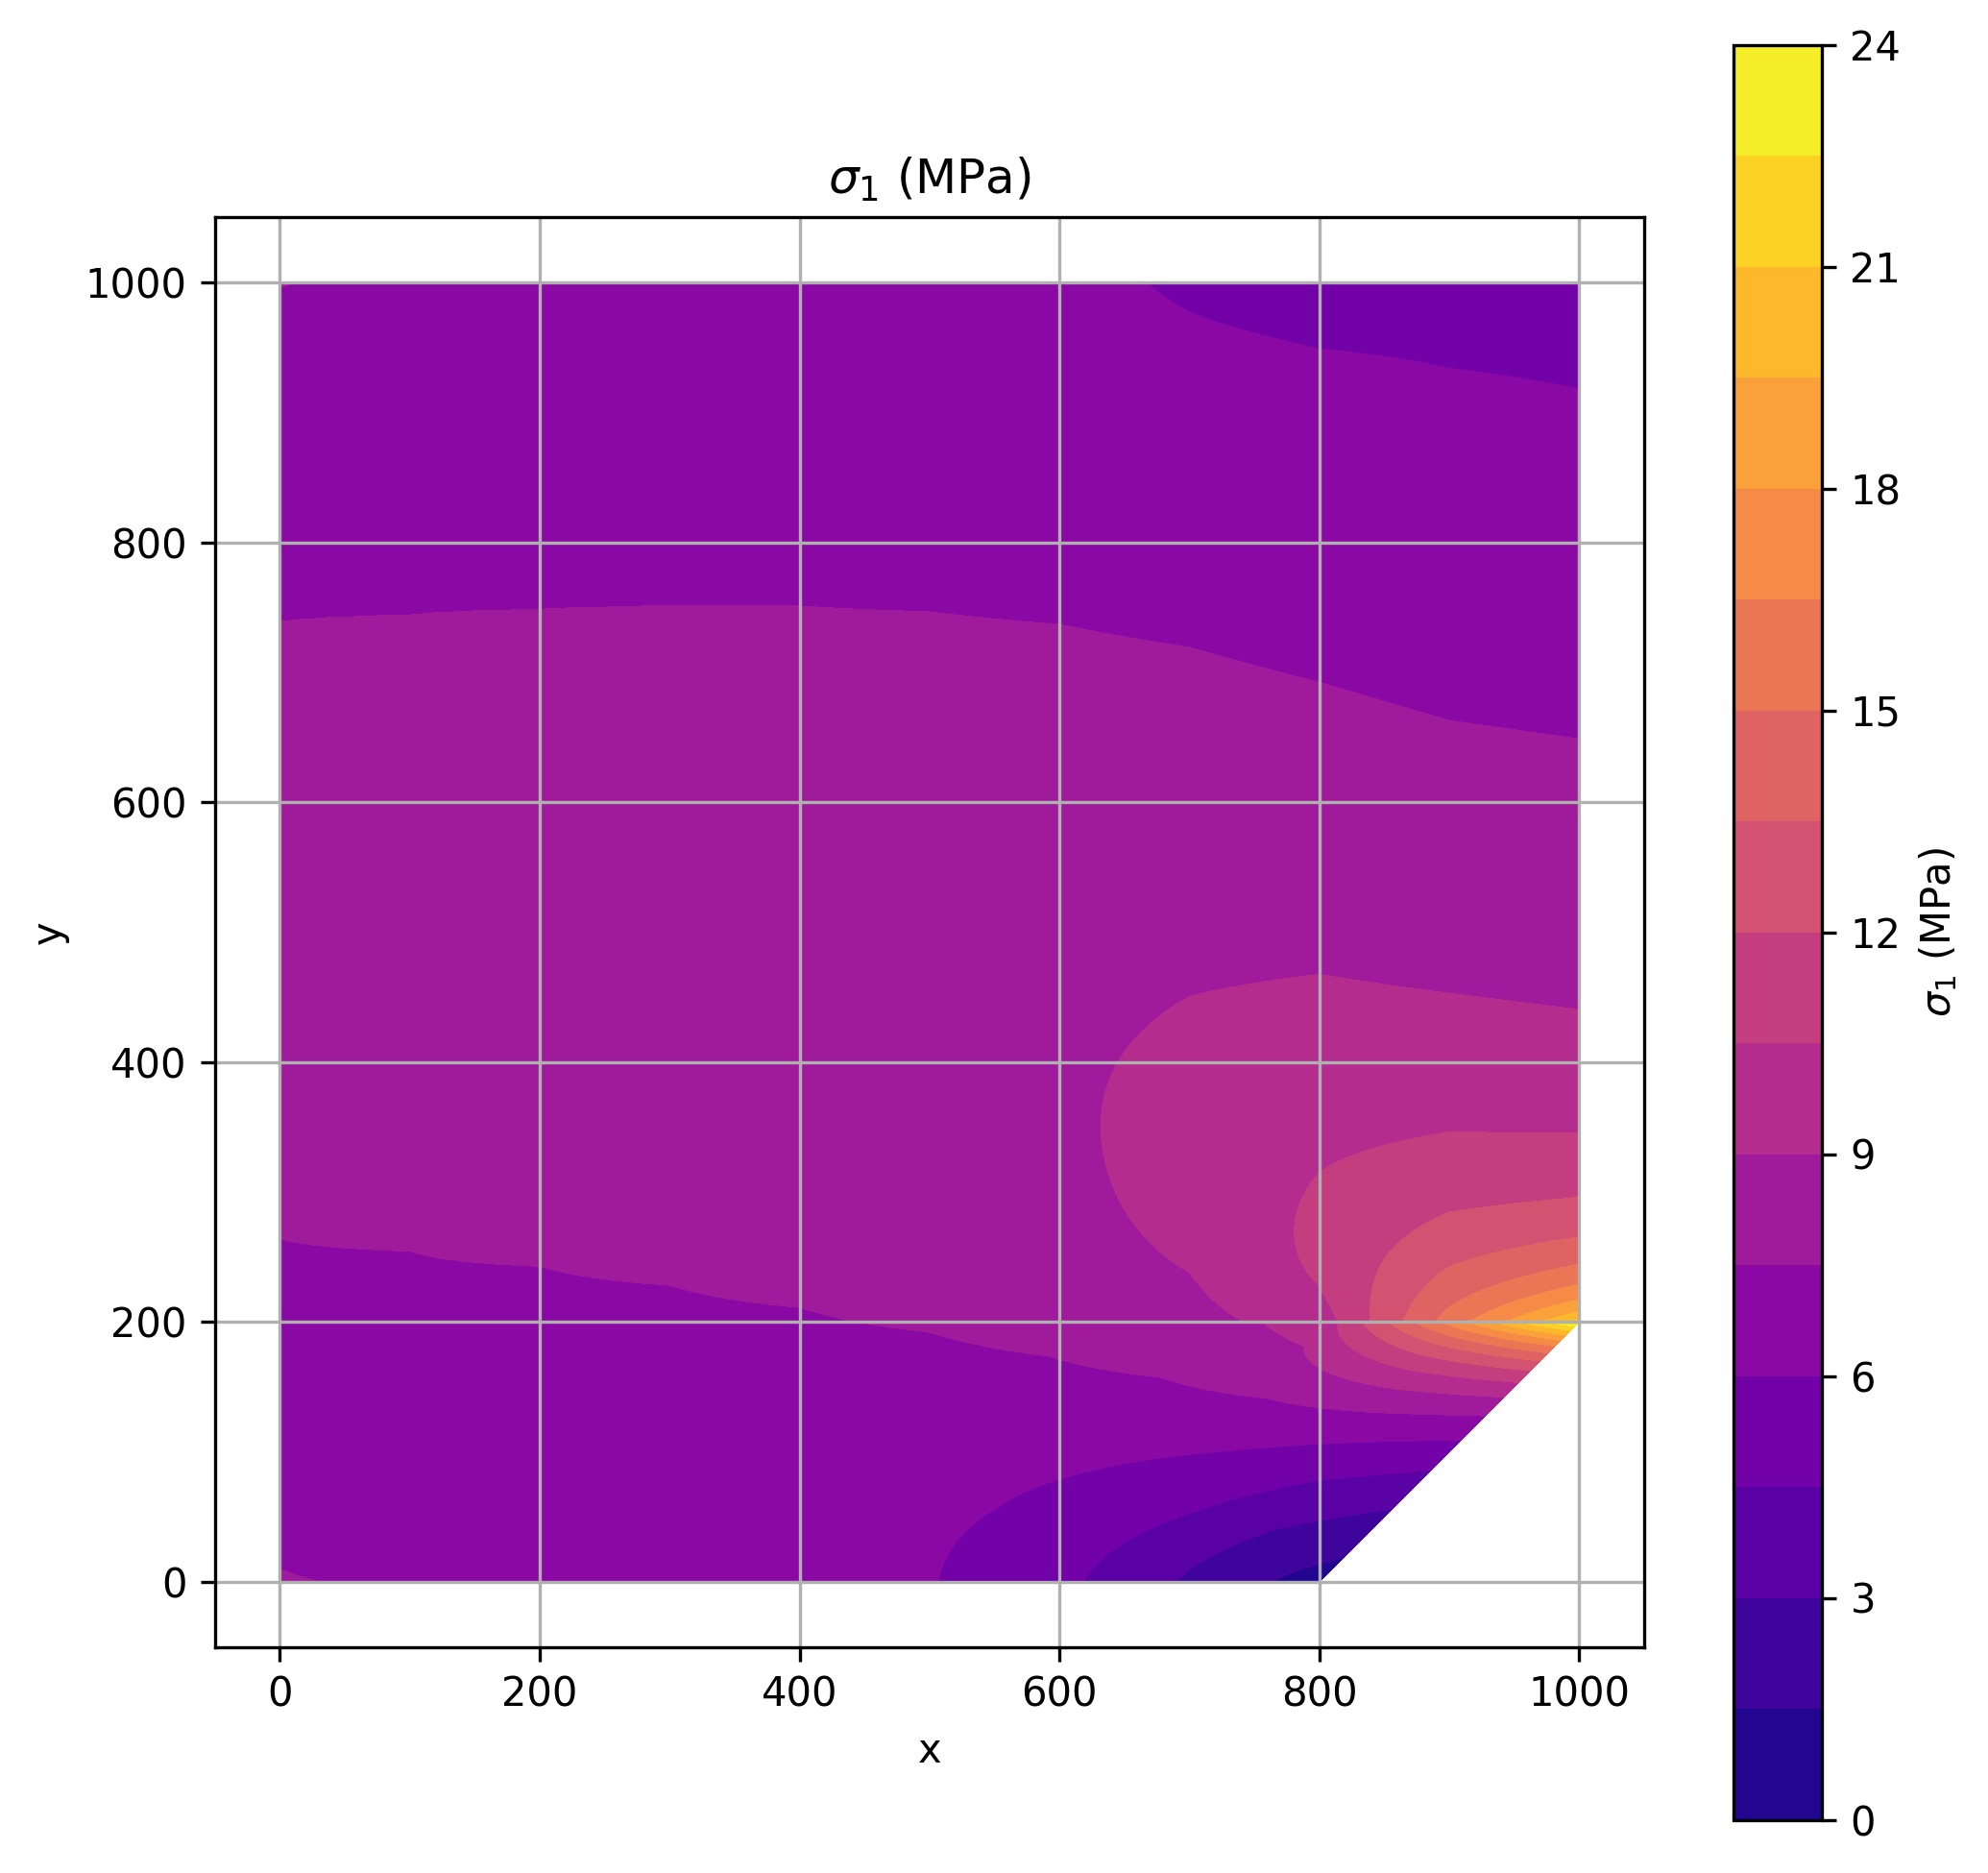
\includegraphics[width=\textwidth]{GRAFICOS/Quad4/1.25mm_global/resultados - sigma_1.png}
    \caption{Local mesh refinement - $h=1.25mm$}
    \label{fig:img23}
  \end{subfigure}
\end{figure}

\subsubsection{Quad9 Element}

In this section, the same procedure was followed, but increasing the order of the mesh elements to Quad9.

\begin{figure}[H]
  \centering
  \begin{subfigure}[b]{0.45\textwidth}
    \centering
    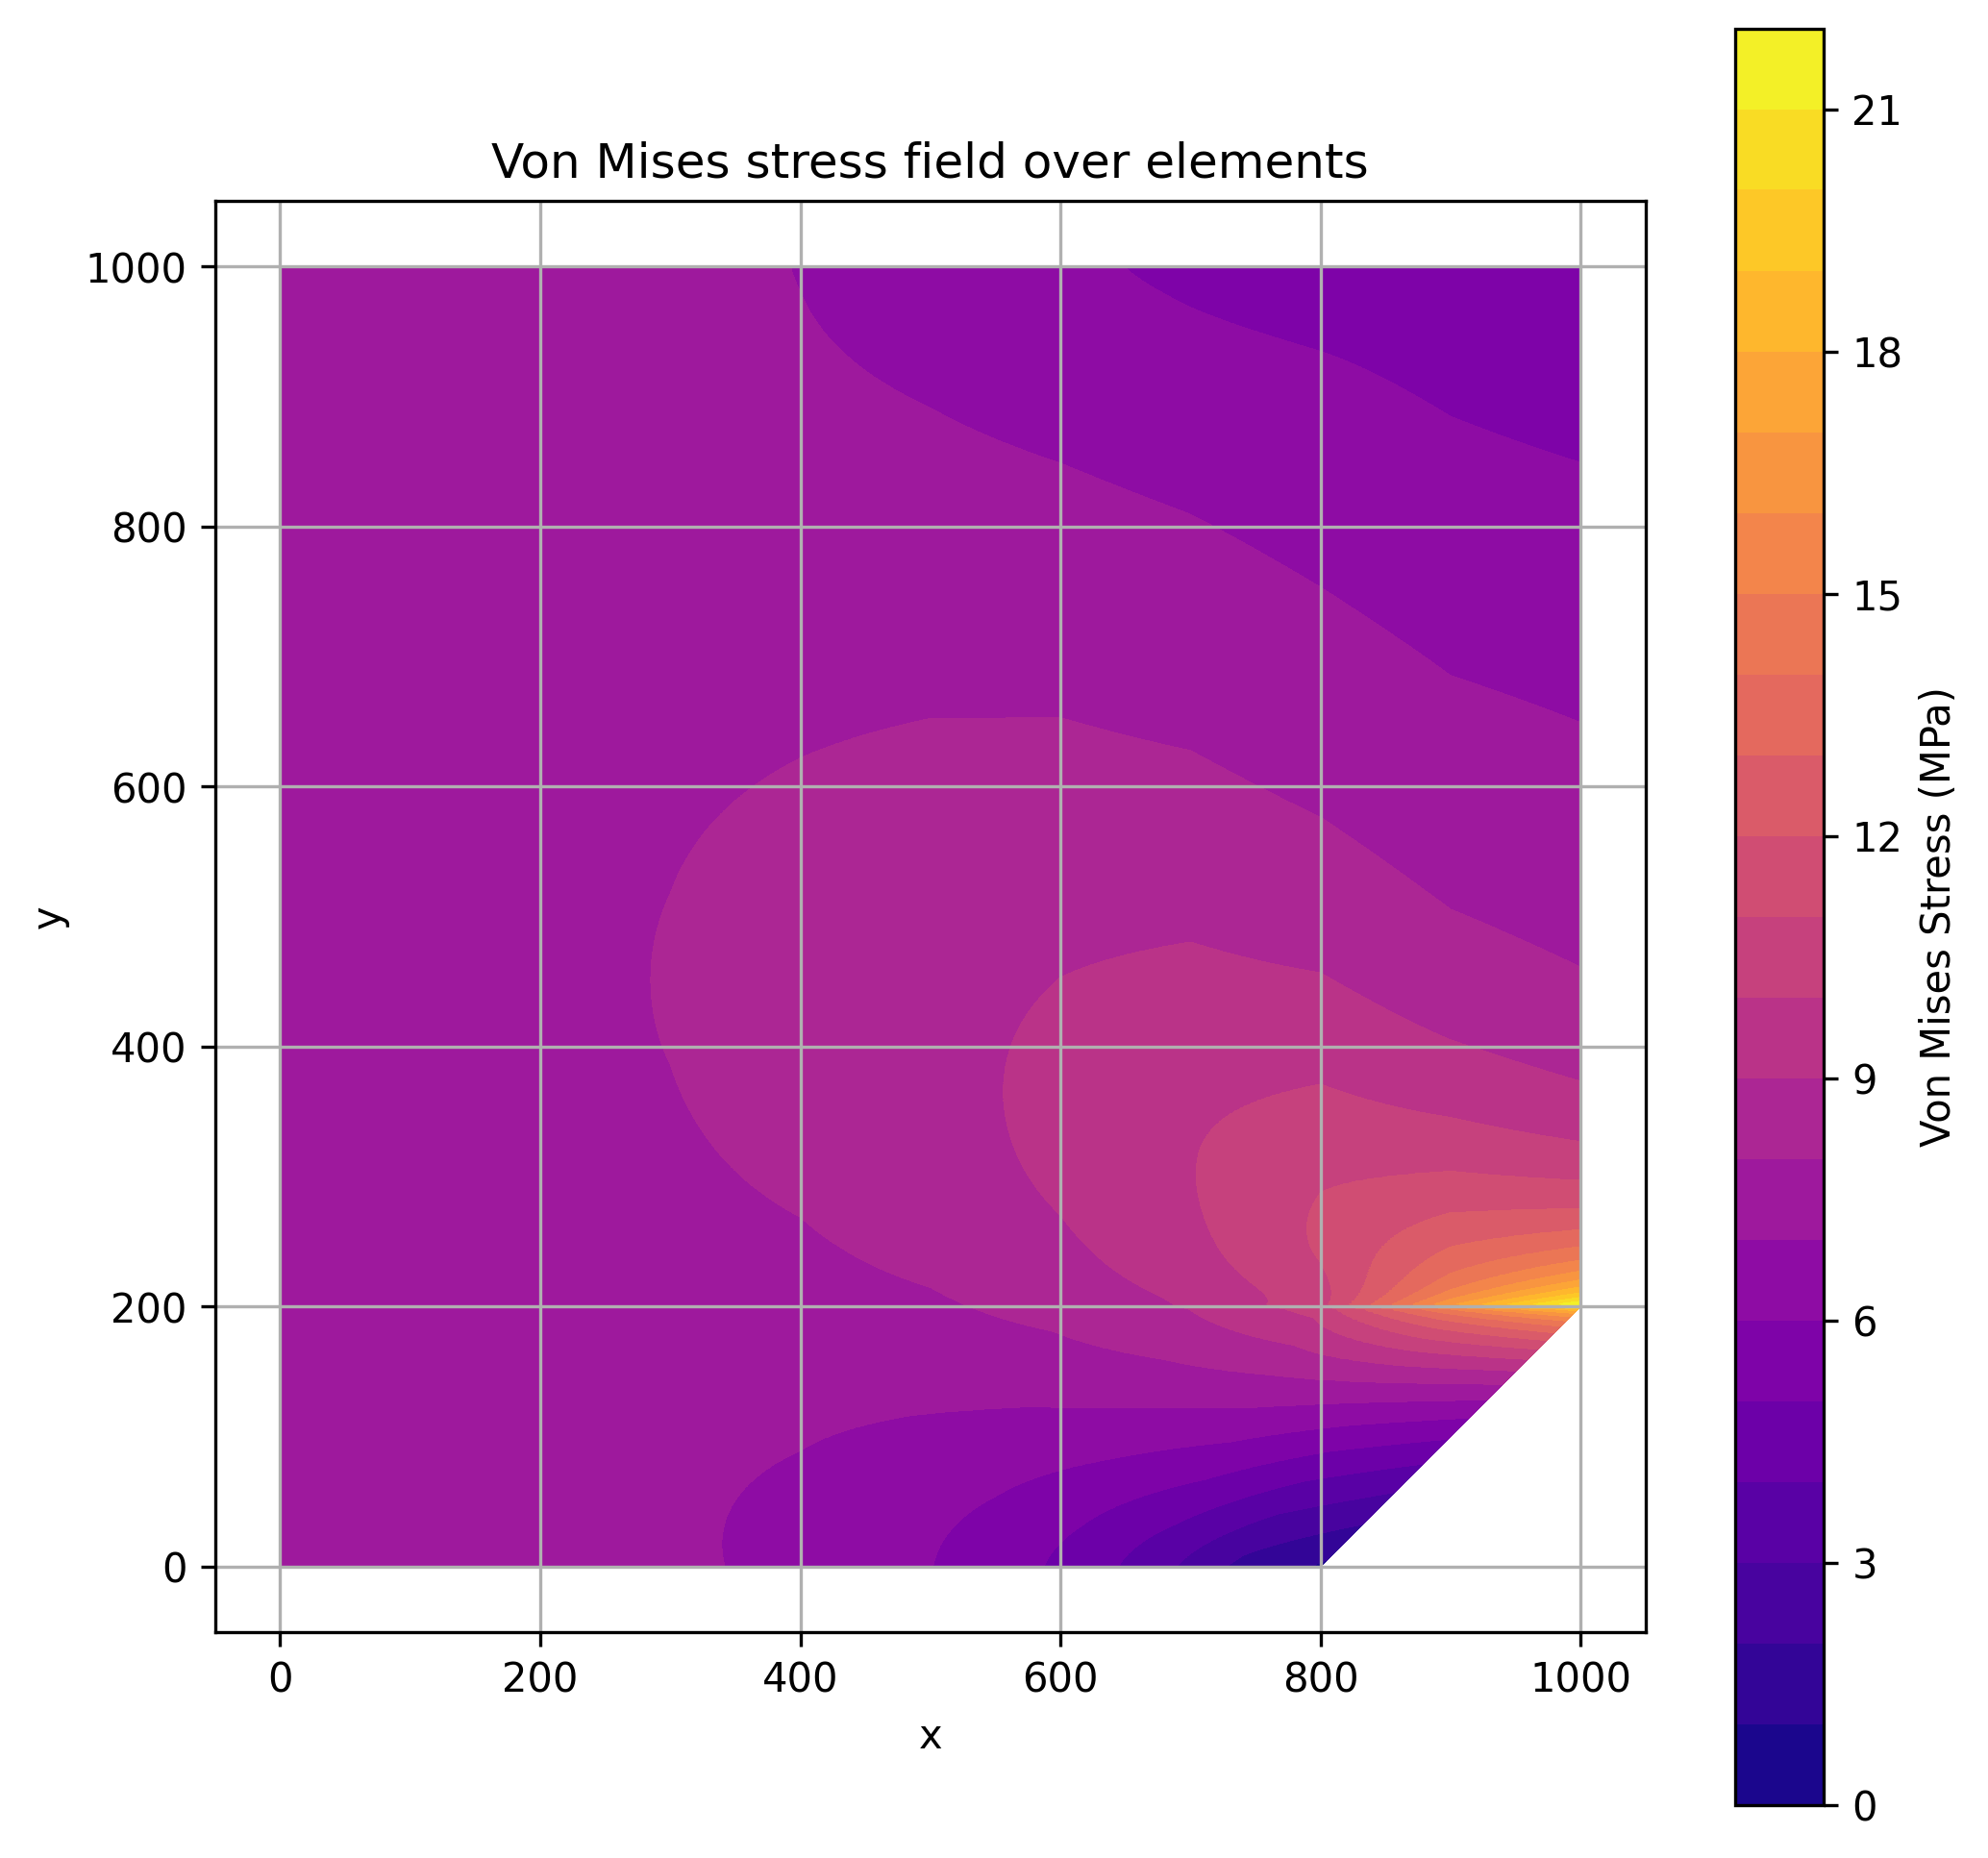
\includegraphics[width=\textwidth]{GRAFICOS/Quad9/2mm_global/resultados_von_mises.png}
    \caption{Global mesh refinement - $h=2mm$}
    \label{fig:img1}
  \end{subfigure}
  \hfill
  \begin{subfigure}[b]{0.45\textwidth}
    \centering
    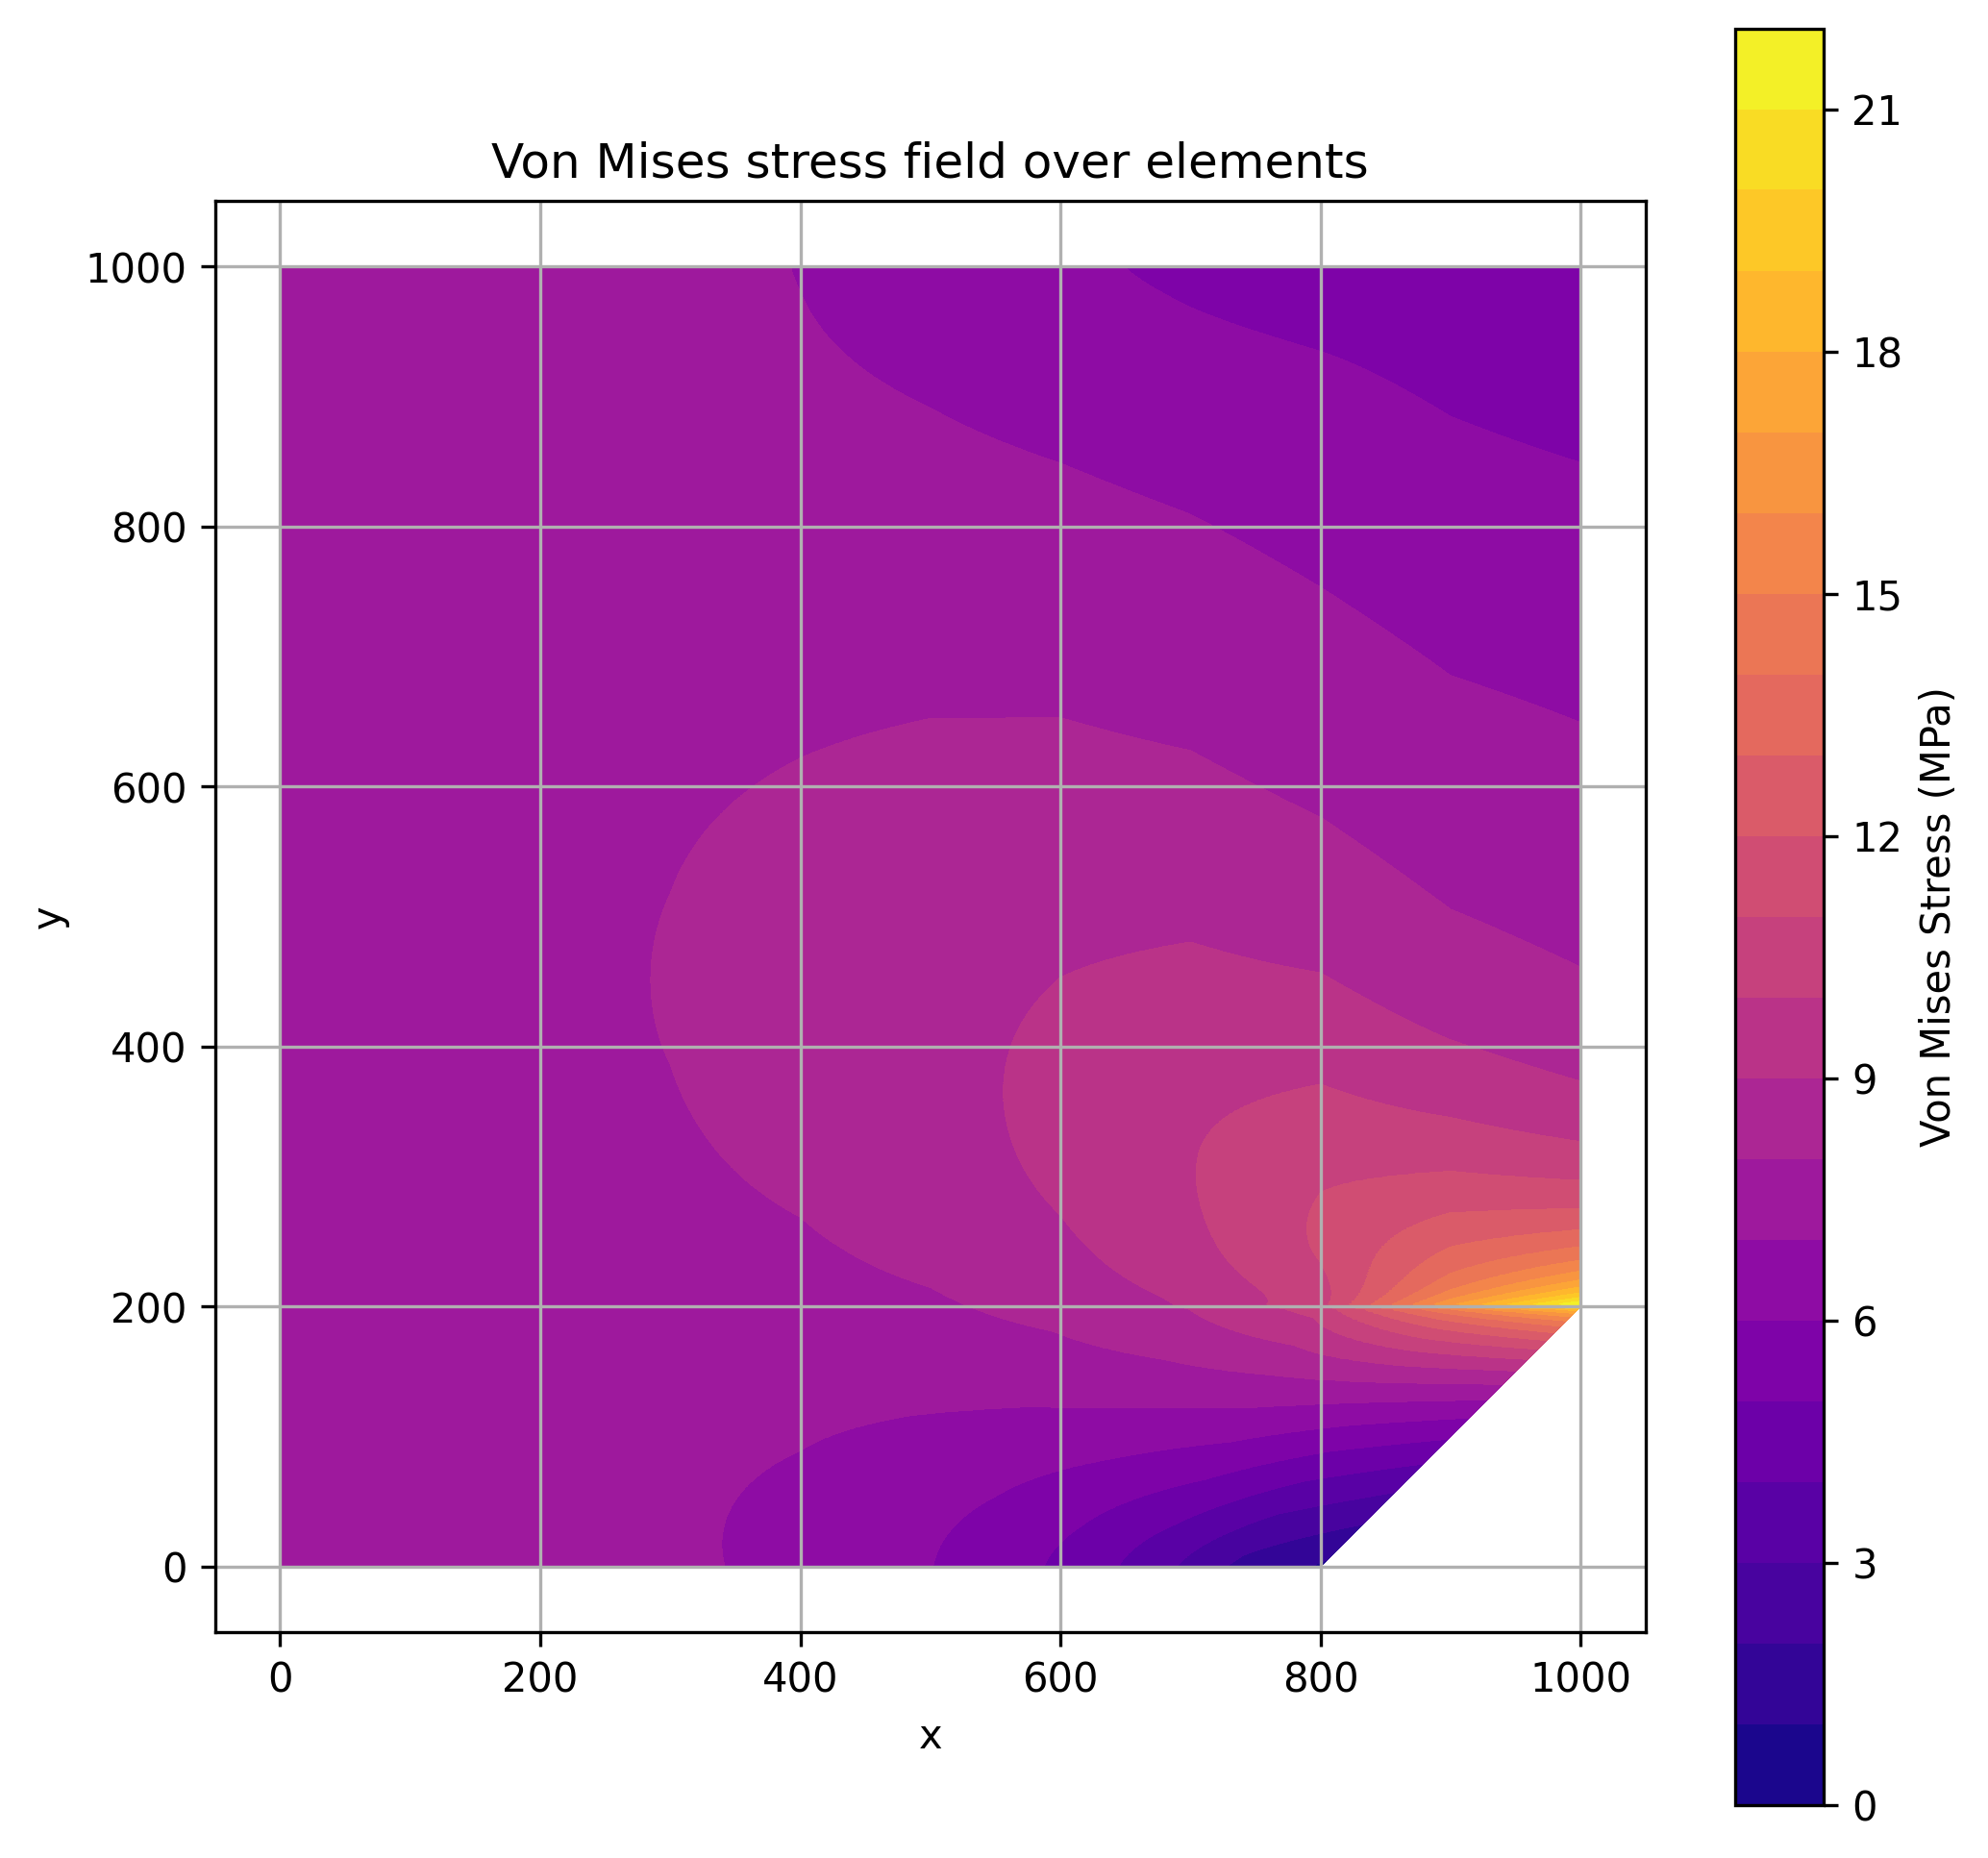
\includegraphics[width=\textwidth]{GRAFICOS/Quad9/2mm_global/resultados_von_mises.png}
    \caption{Local mesh refinement - $h=2mm$}
    \label{fig:img2}
  \end{subfigure}
\end{figure}

\begin{figure}[H]
  \centering
  \begin{subfigure}[b]{0.45\textwidth}
    \centering
    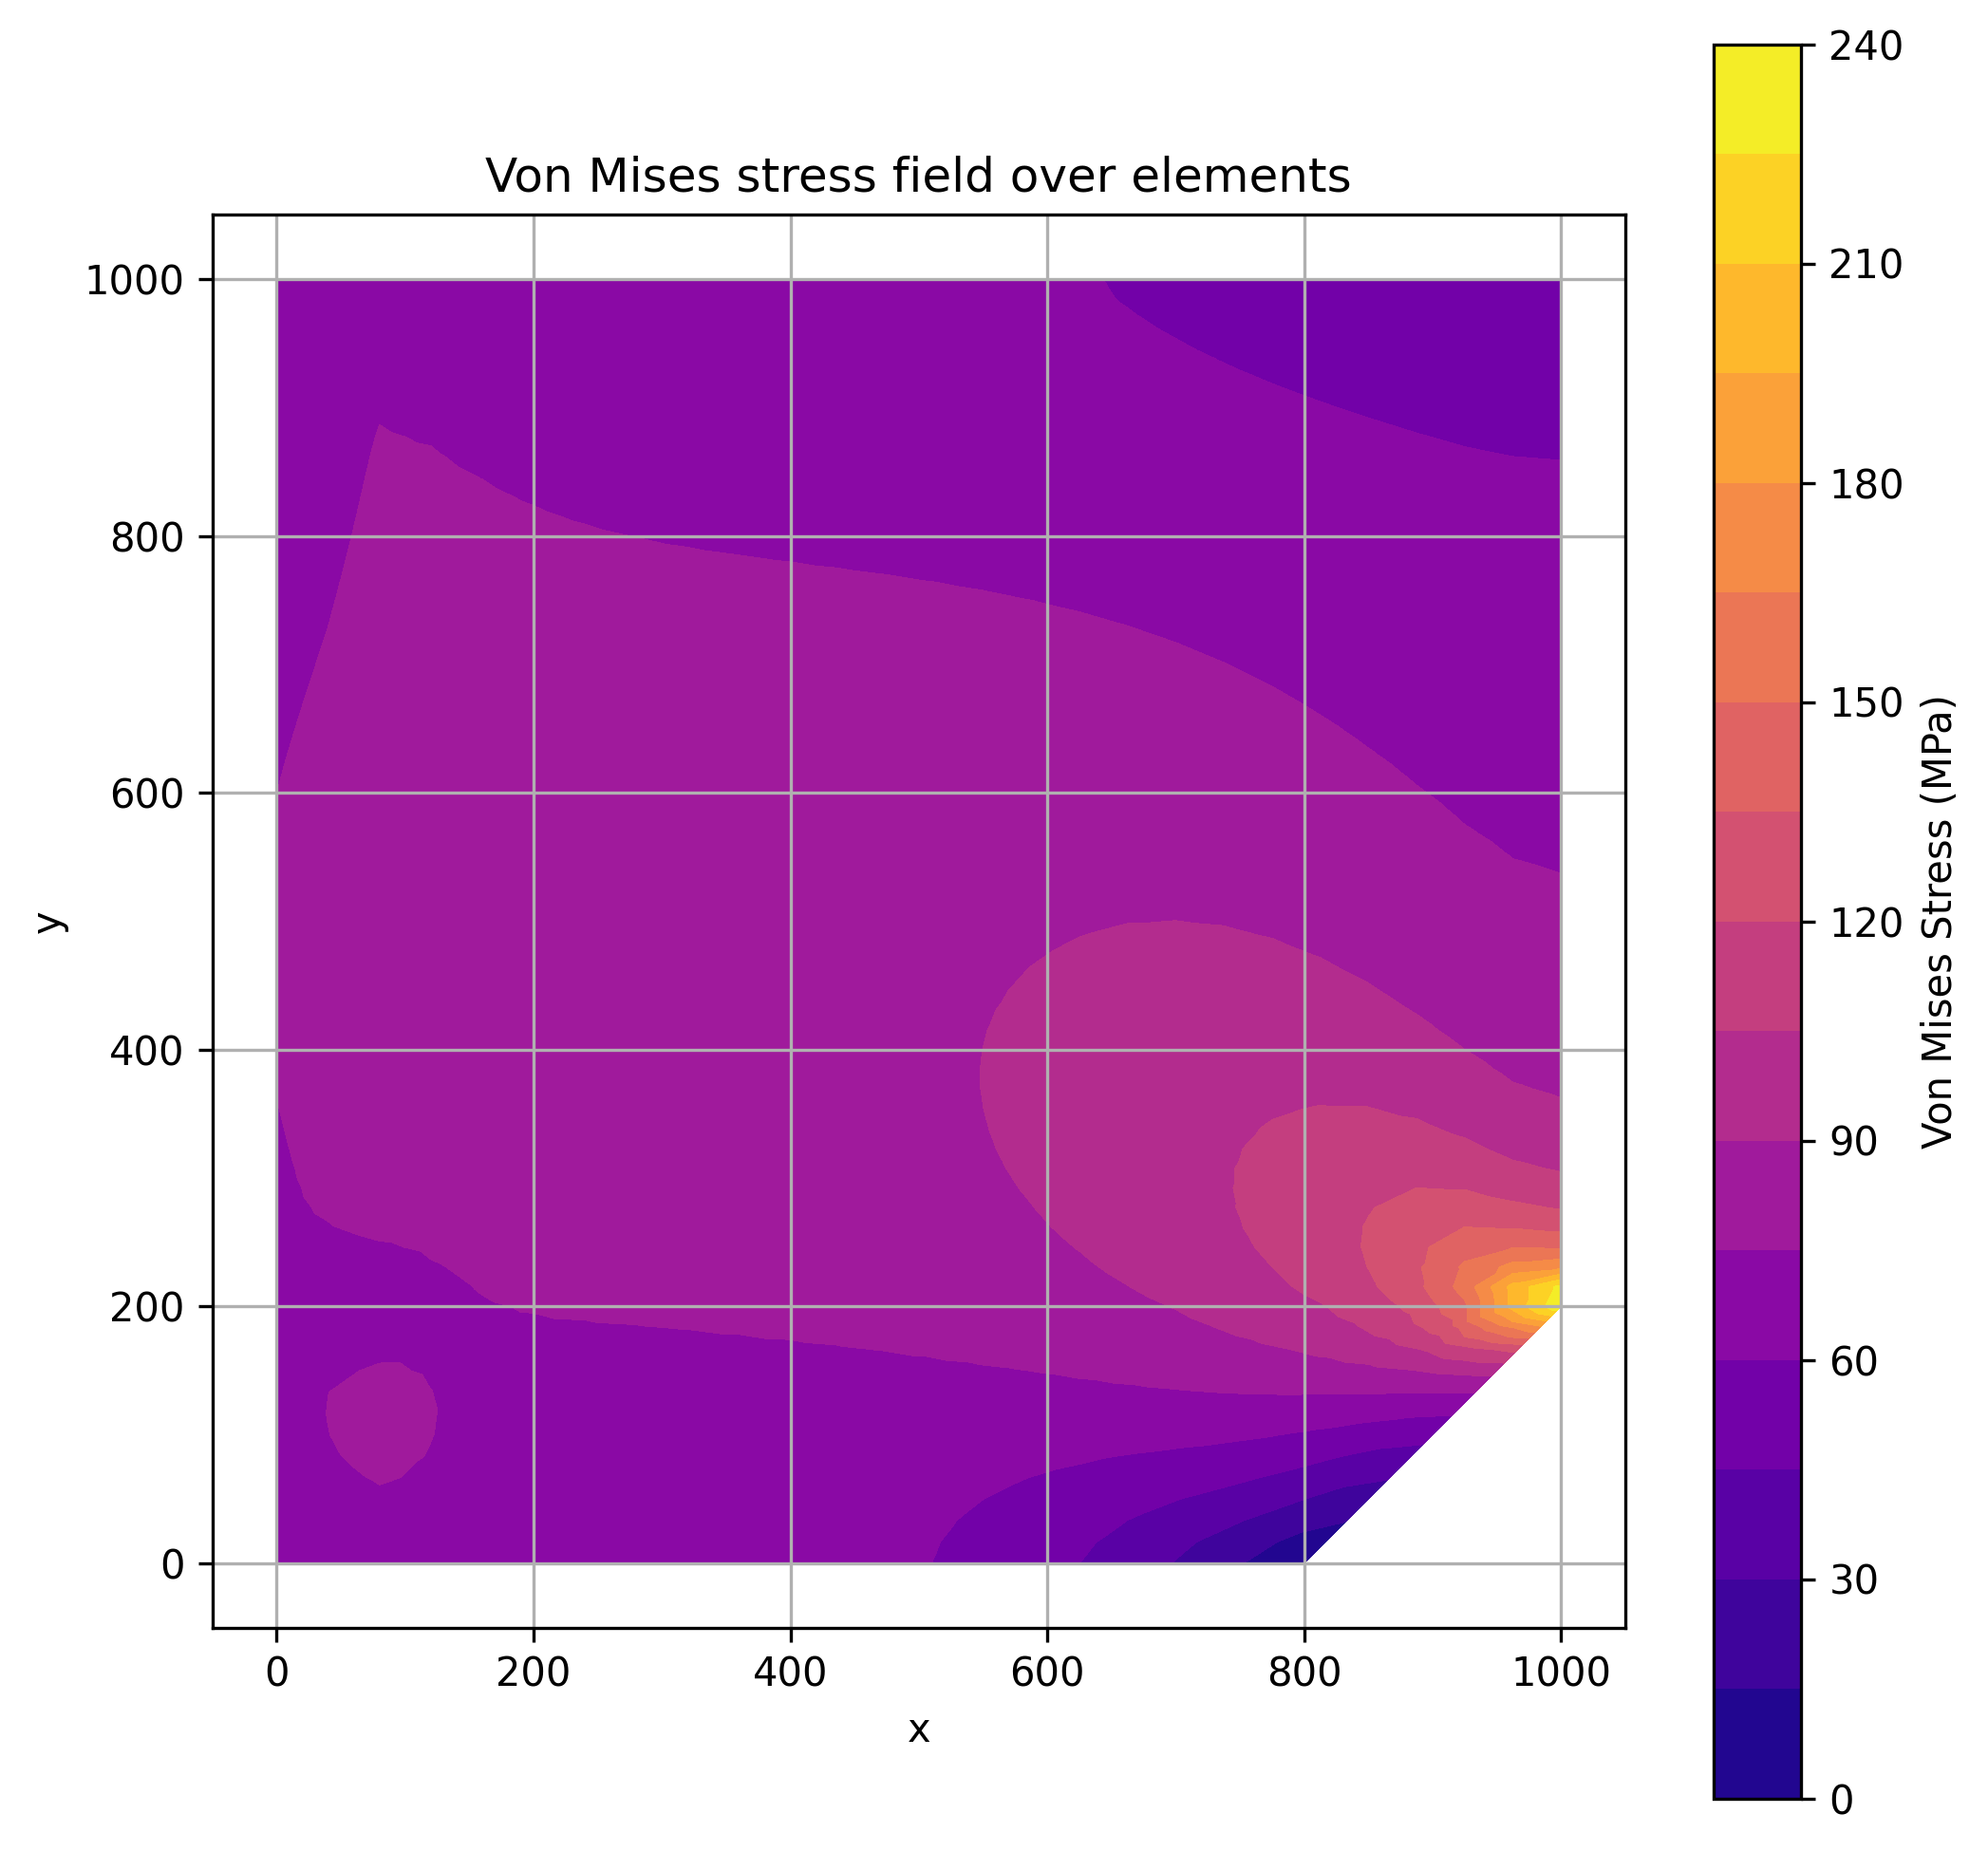
\includegraphics[width=\textwidth]{GRAFICOS/Quad9/1.75mm_global/resultados_von_mises.png}
    \caption{Global mesh refinement - $h=1.75mm$}
    \label{fig:img11}
  \end{subfigure}
  \hfill
  \begin{subfigure}[b]{0.45\textwidth}
    \centering
    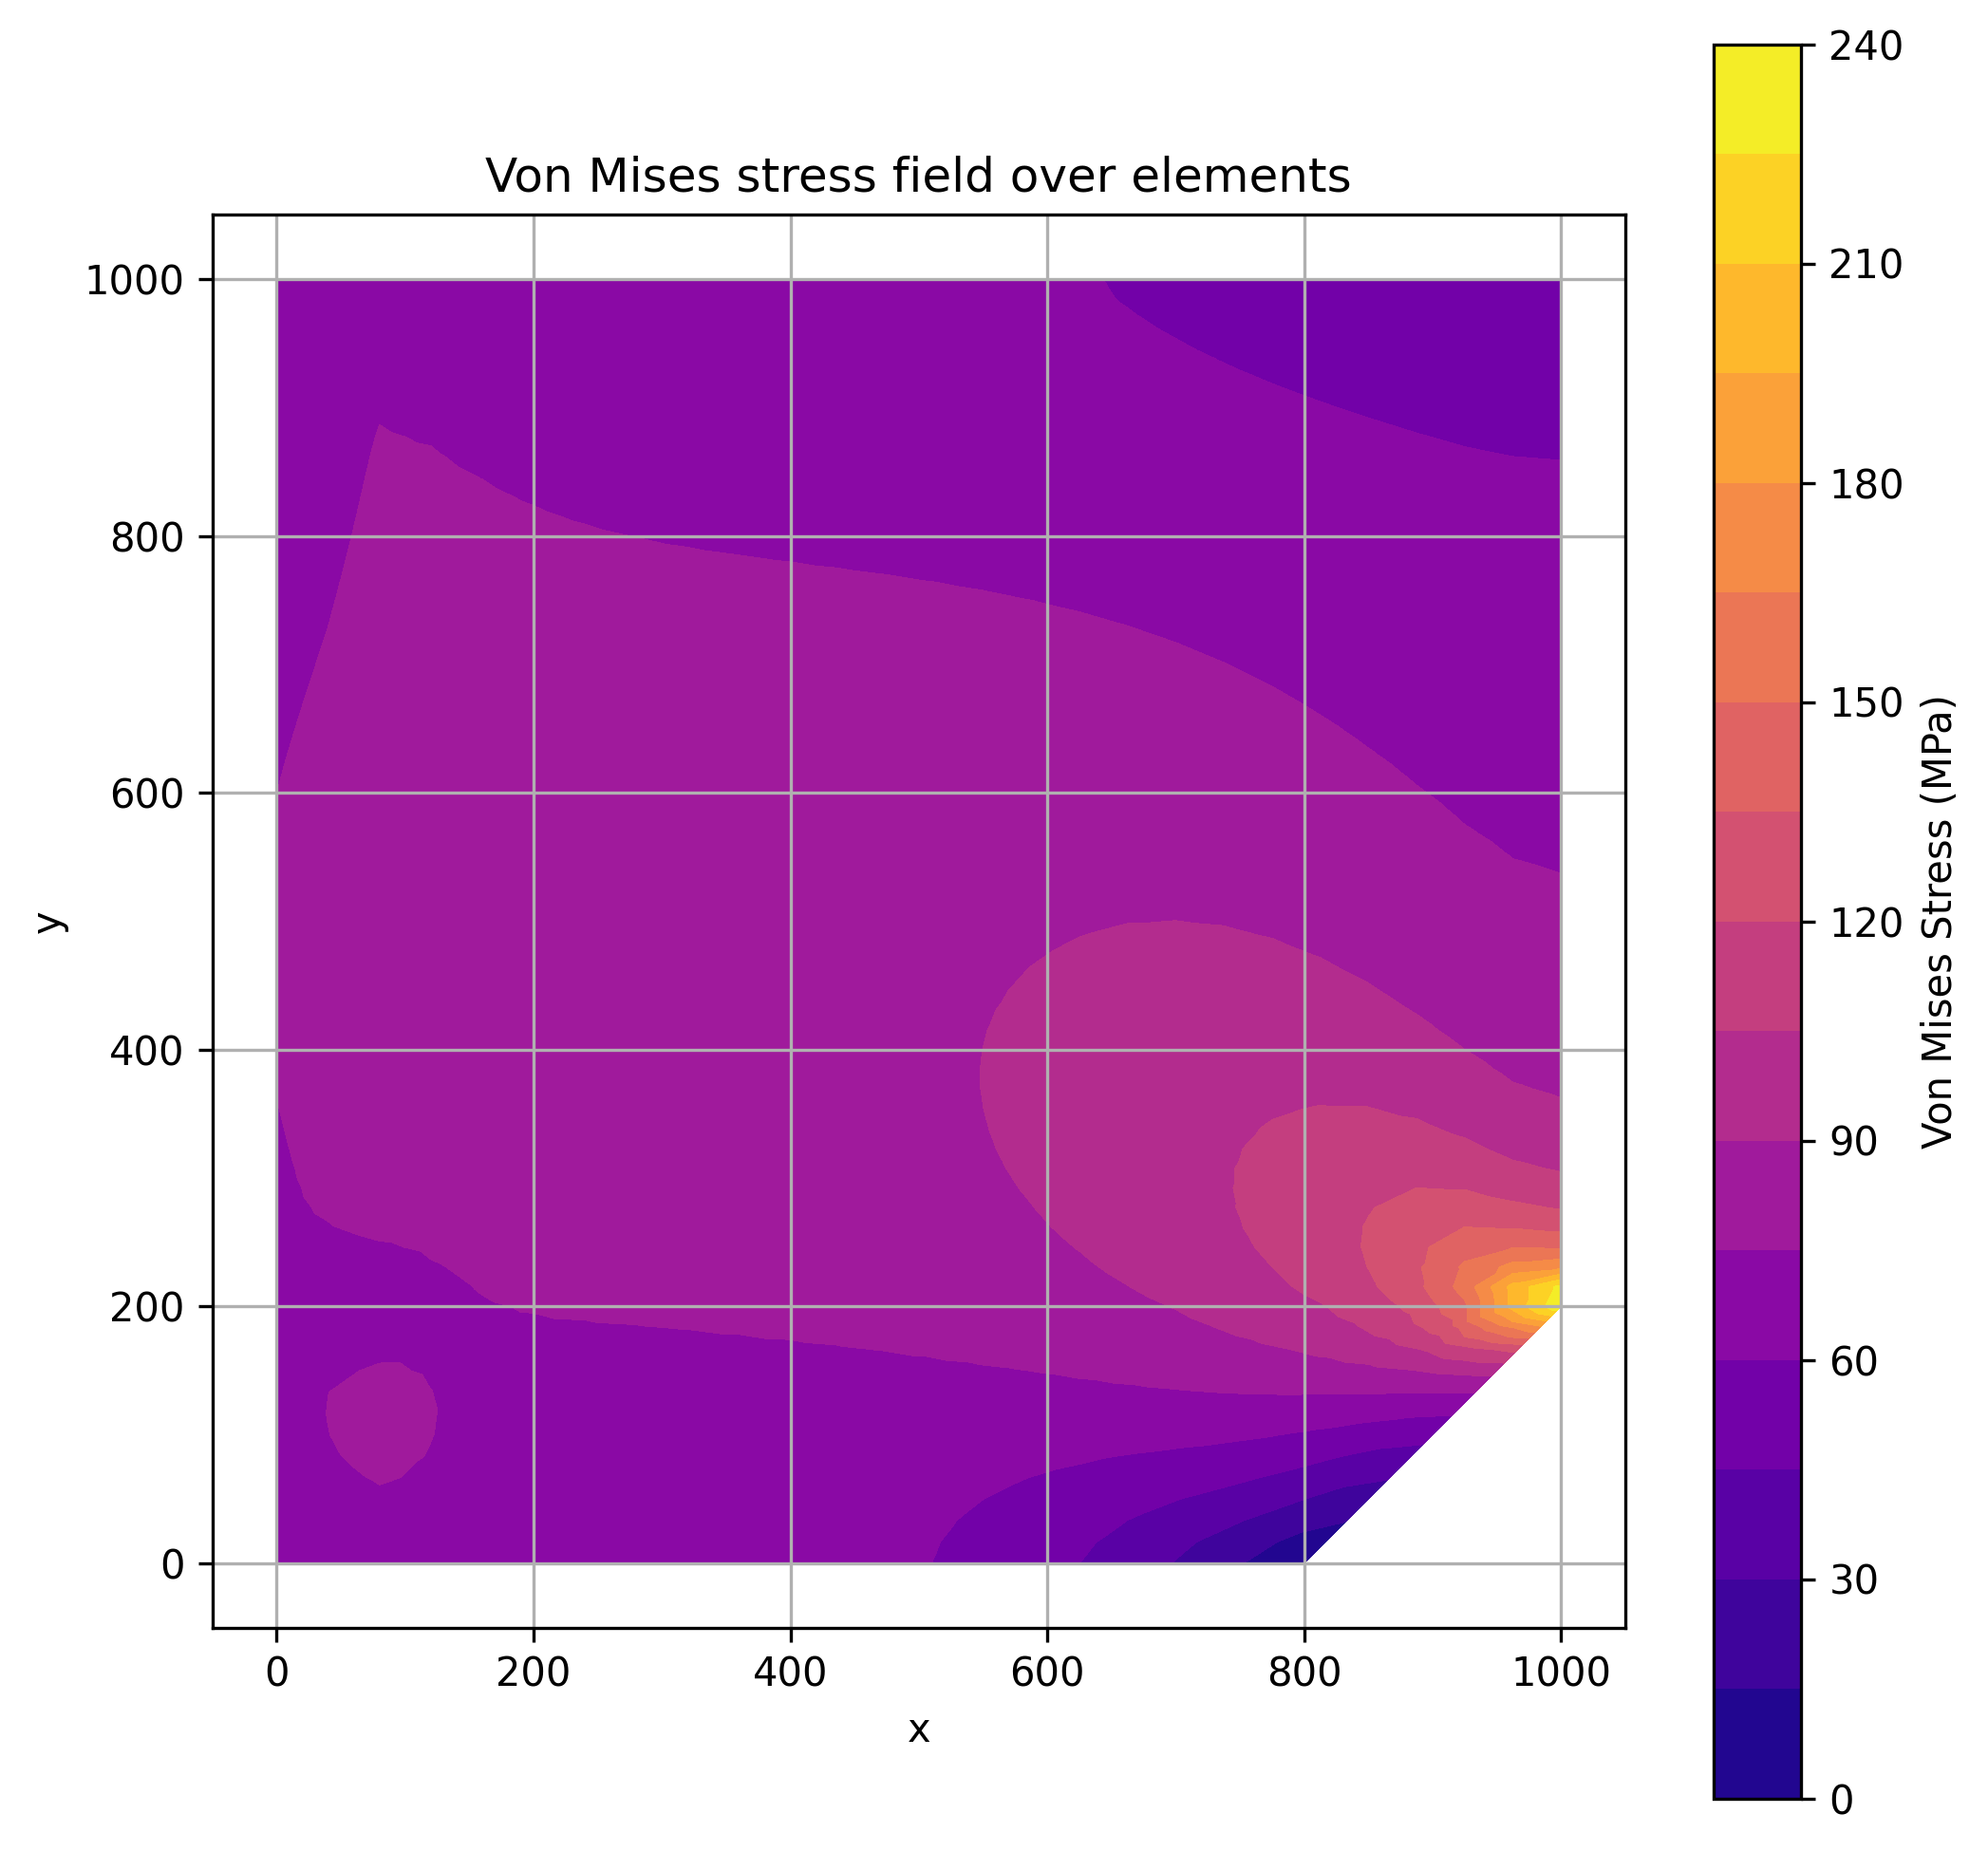
\includegraphics[width=\textwidth]{GRAFICOS/Quad9/1.75mm_global/resultados_von_mises.png}
    \caption{Local mesh refinement - $h=1.75mm$}
    \label{fig:img21}
  \end{subfigure}
\end{figure}

\begin{figure}[H]
  \centering
  \begin{subfigure}[b]{0.45\textwidth}
    \centering
    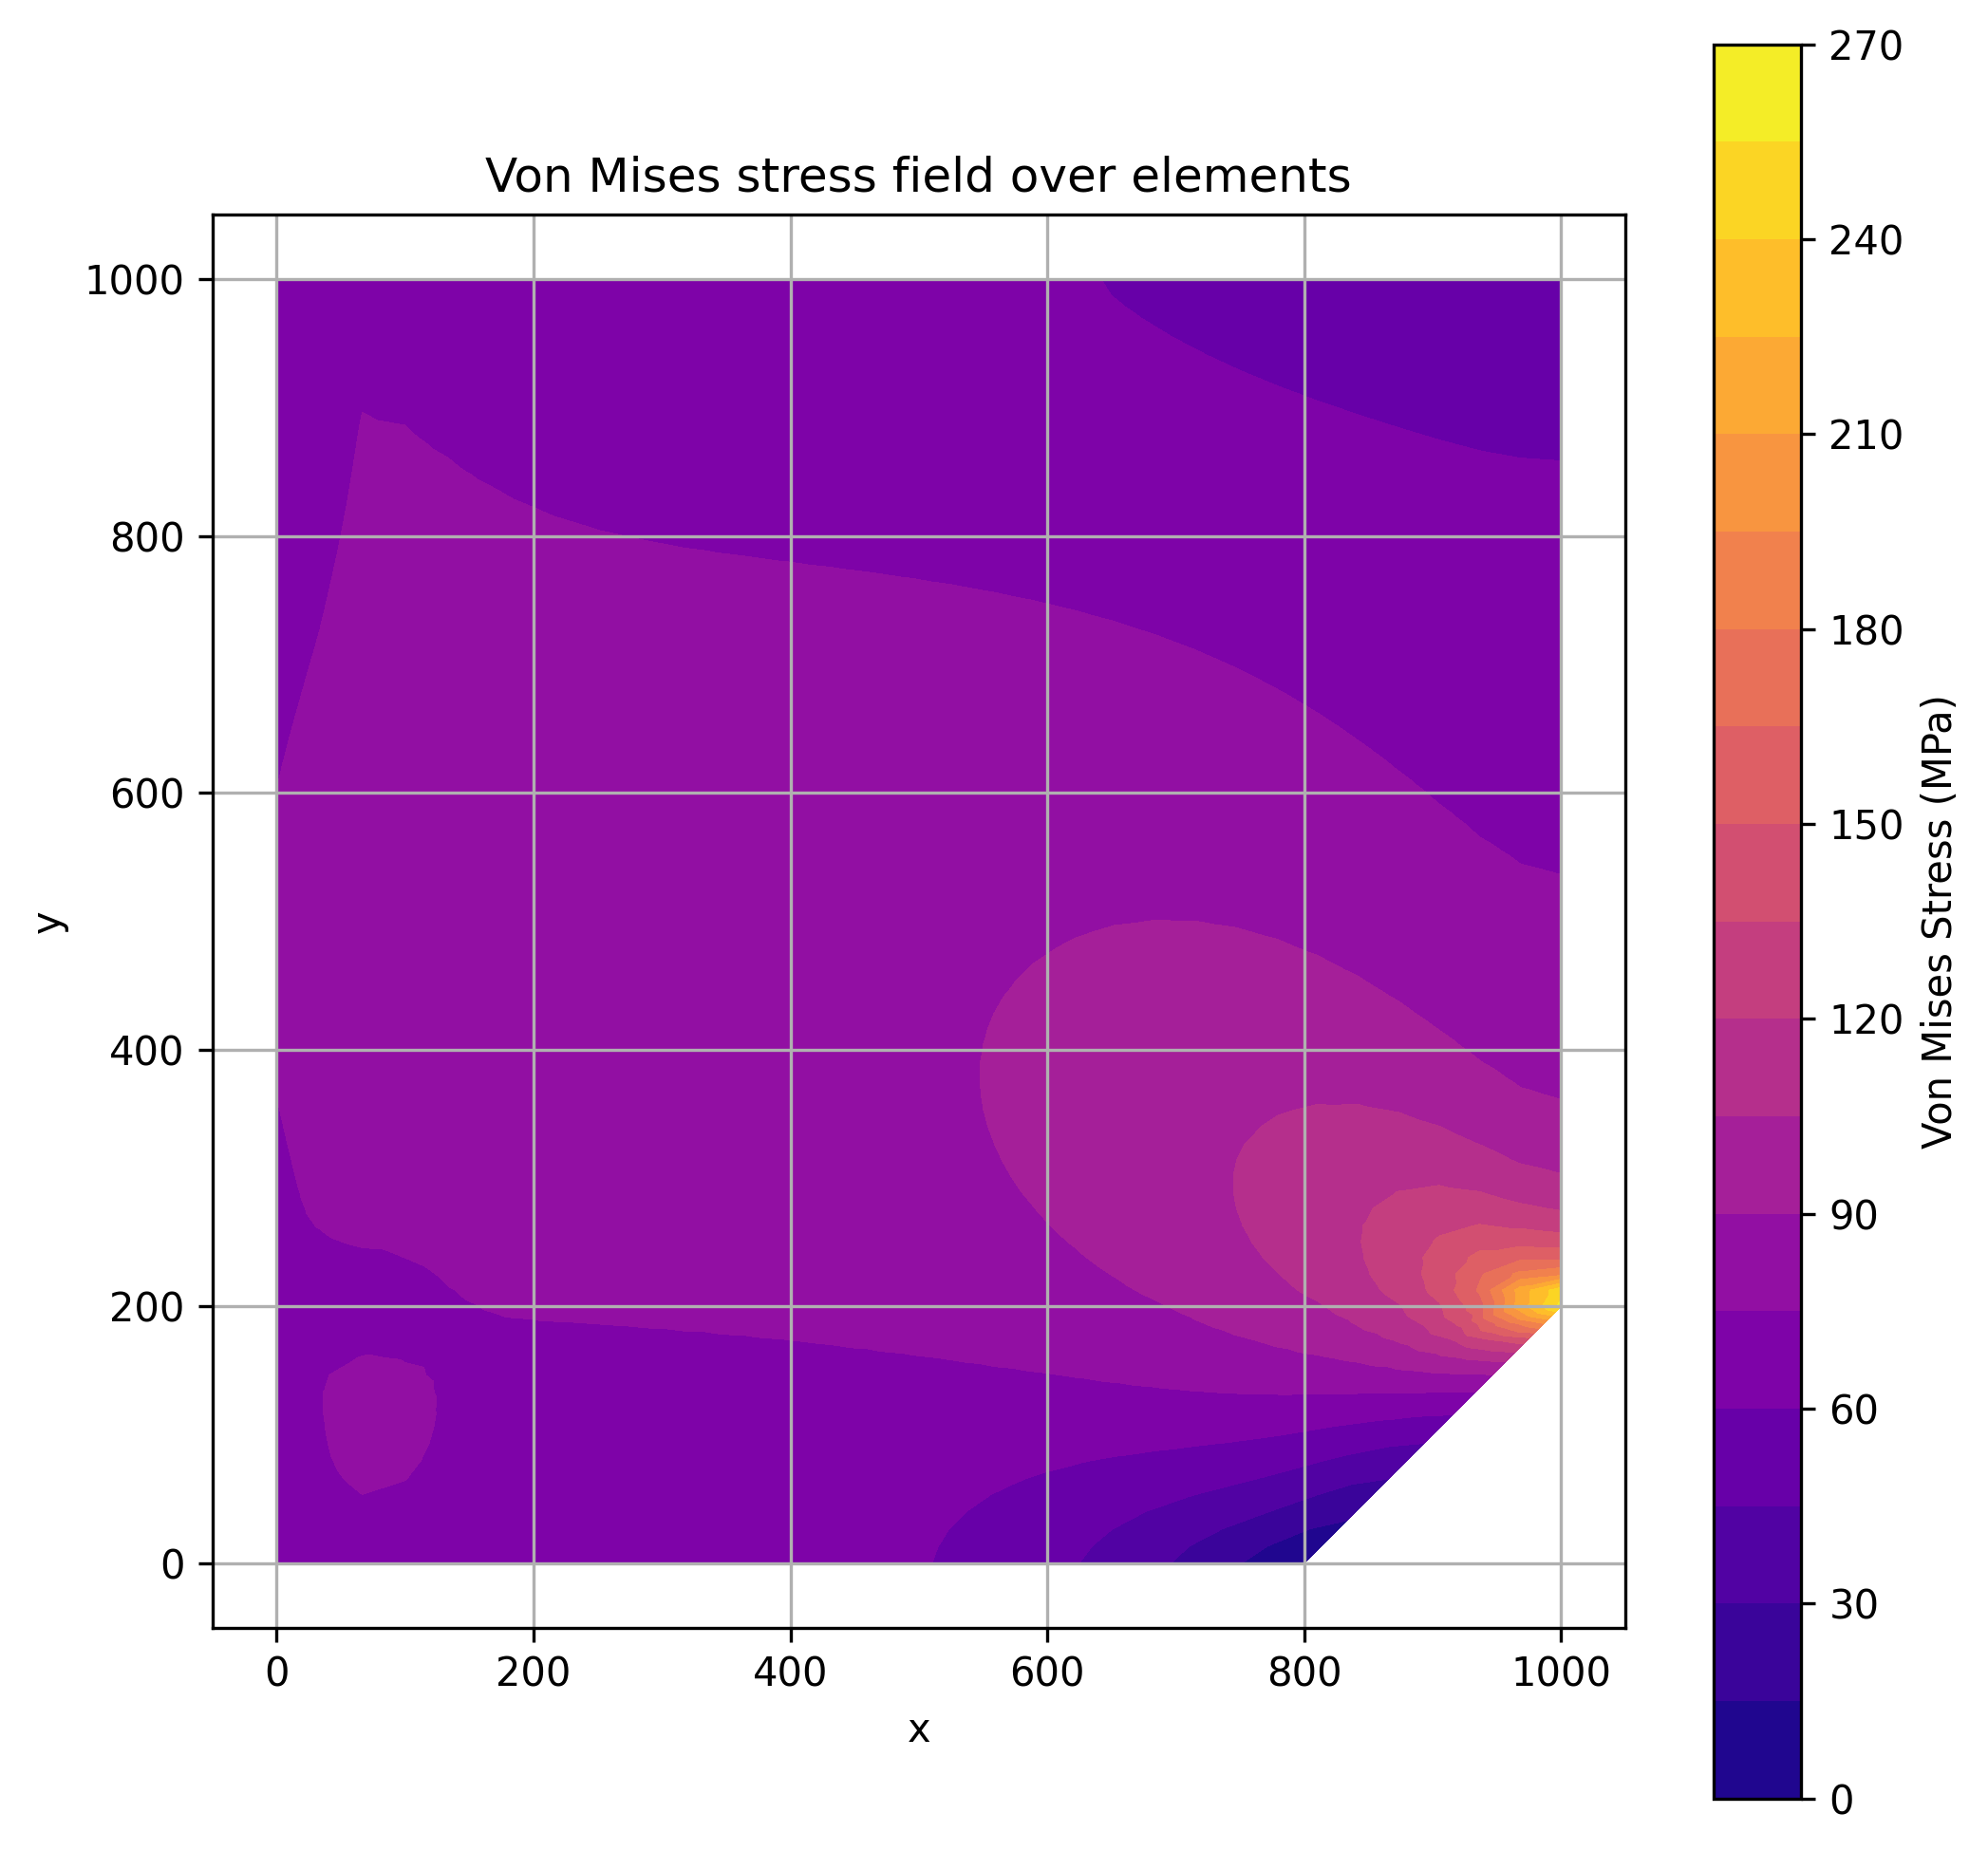
\includegraphics[width=\textwidth]{GRAFICOS/Quad9/1.5mm_global/resultados_von_mises.png}
    \caption{Global mesh refinement - $h=1.5mm$}
    \label{fig:img12}
  \end{subfigure}
  \hfill
  \begin{subfigure}[b]{0.45\textwidth}
    \centering
    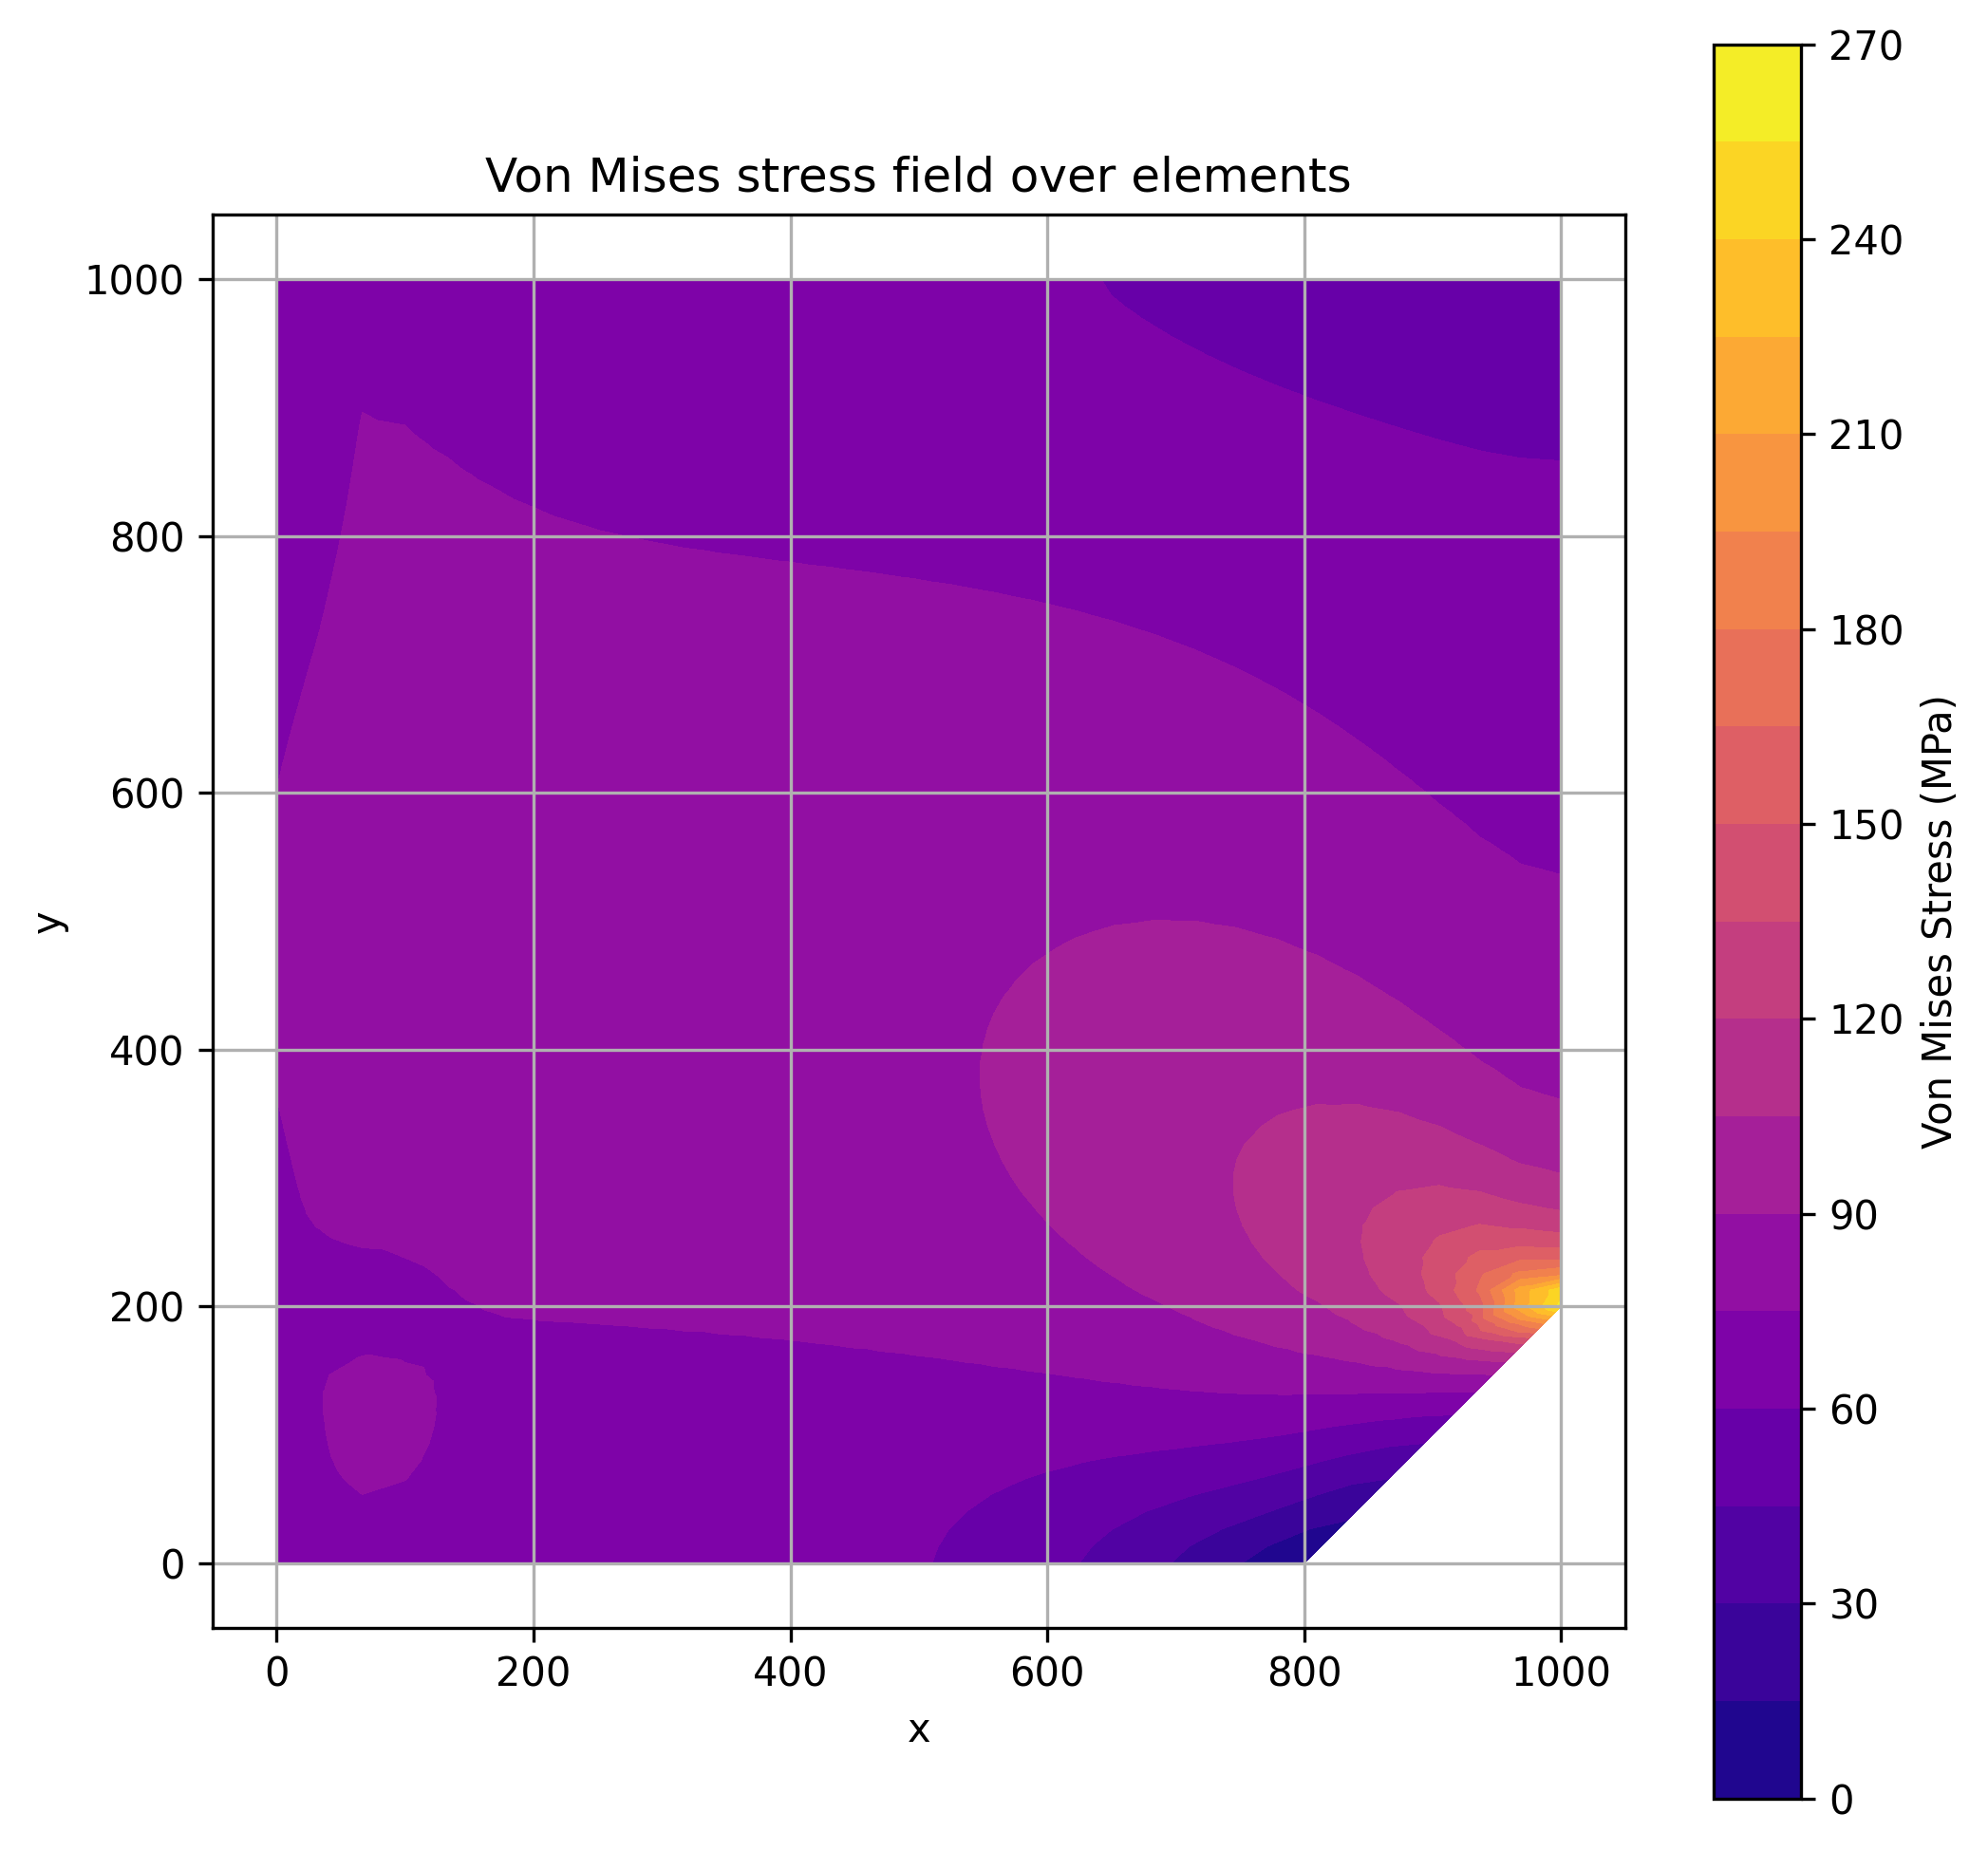
\includegraphics[width=\textwidth]{GRAFICOS/Quad9/1.5mm_global/resultados_von_mises.png}
    \caption{Local mesh refinement - $h=1.5mm$}
    \label{fig:img22}
  \end{subfigure}
\end{figure}

\begin{figure}[H]
  \centering
  \begin{subfigure}[b]{0.45\textwidth}
    \centering
    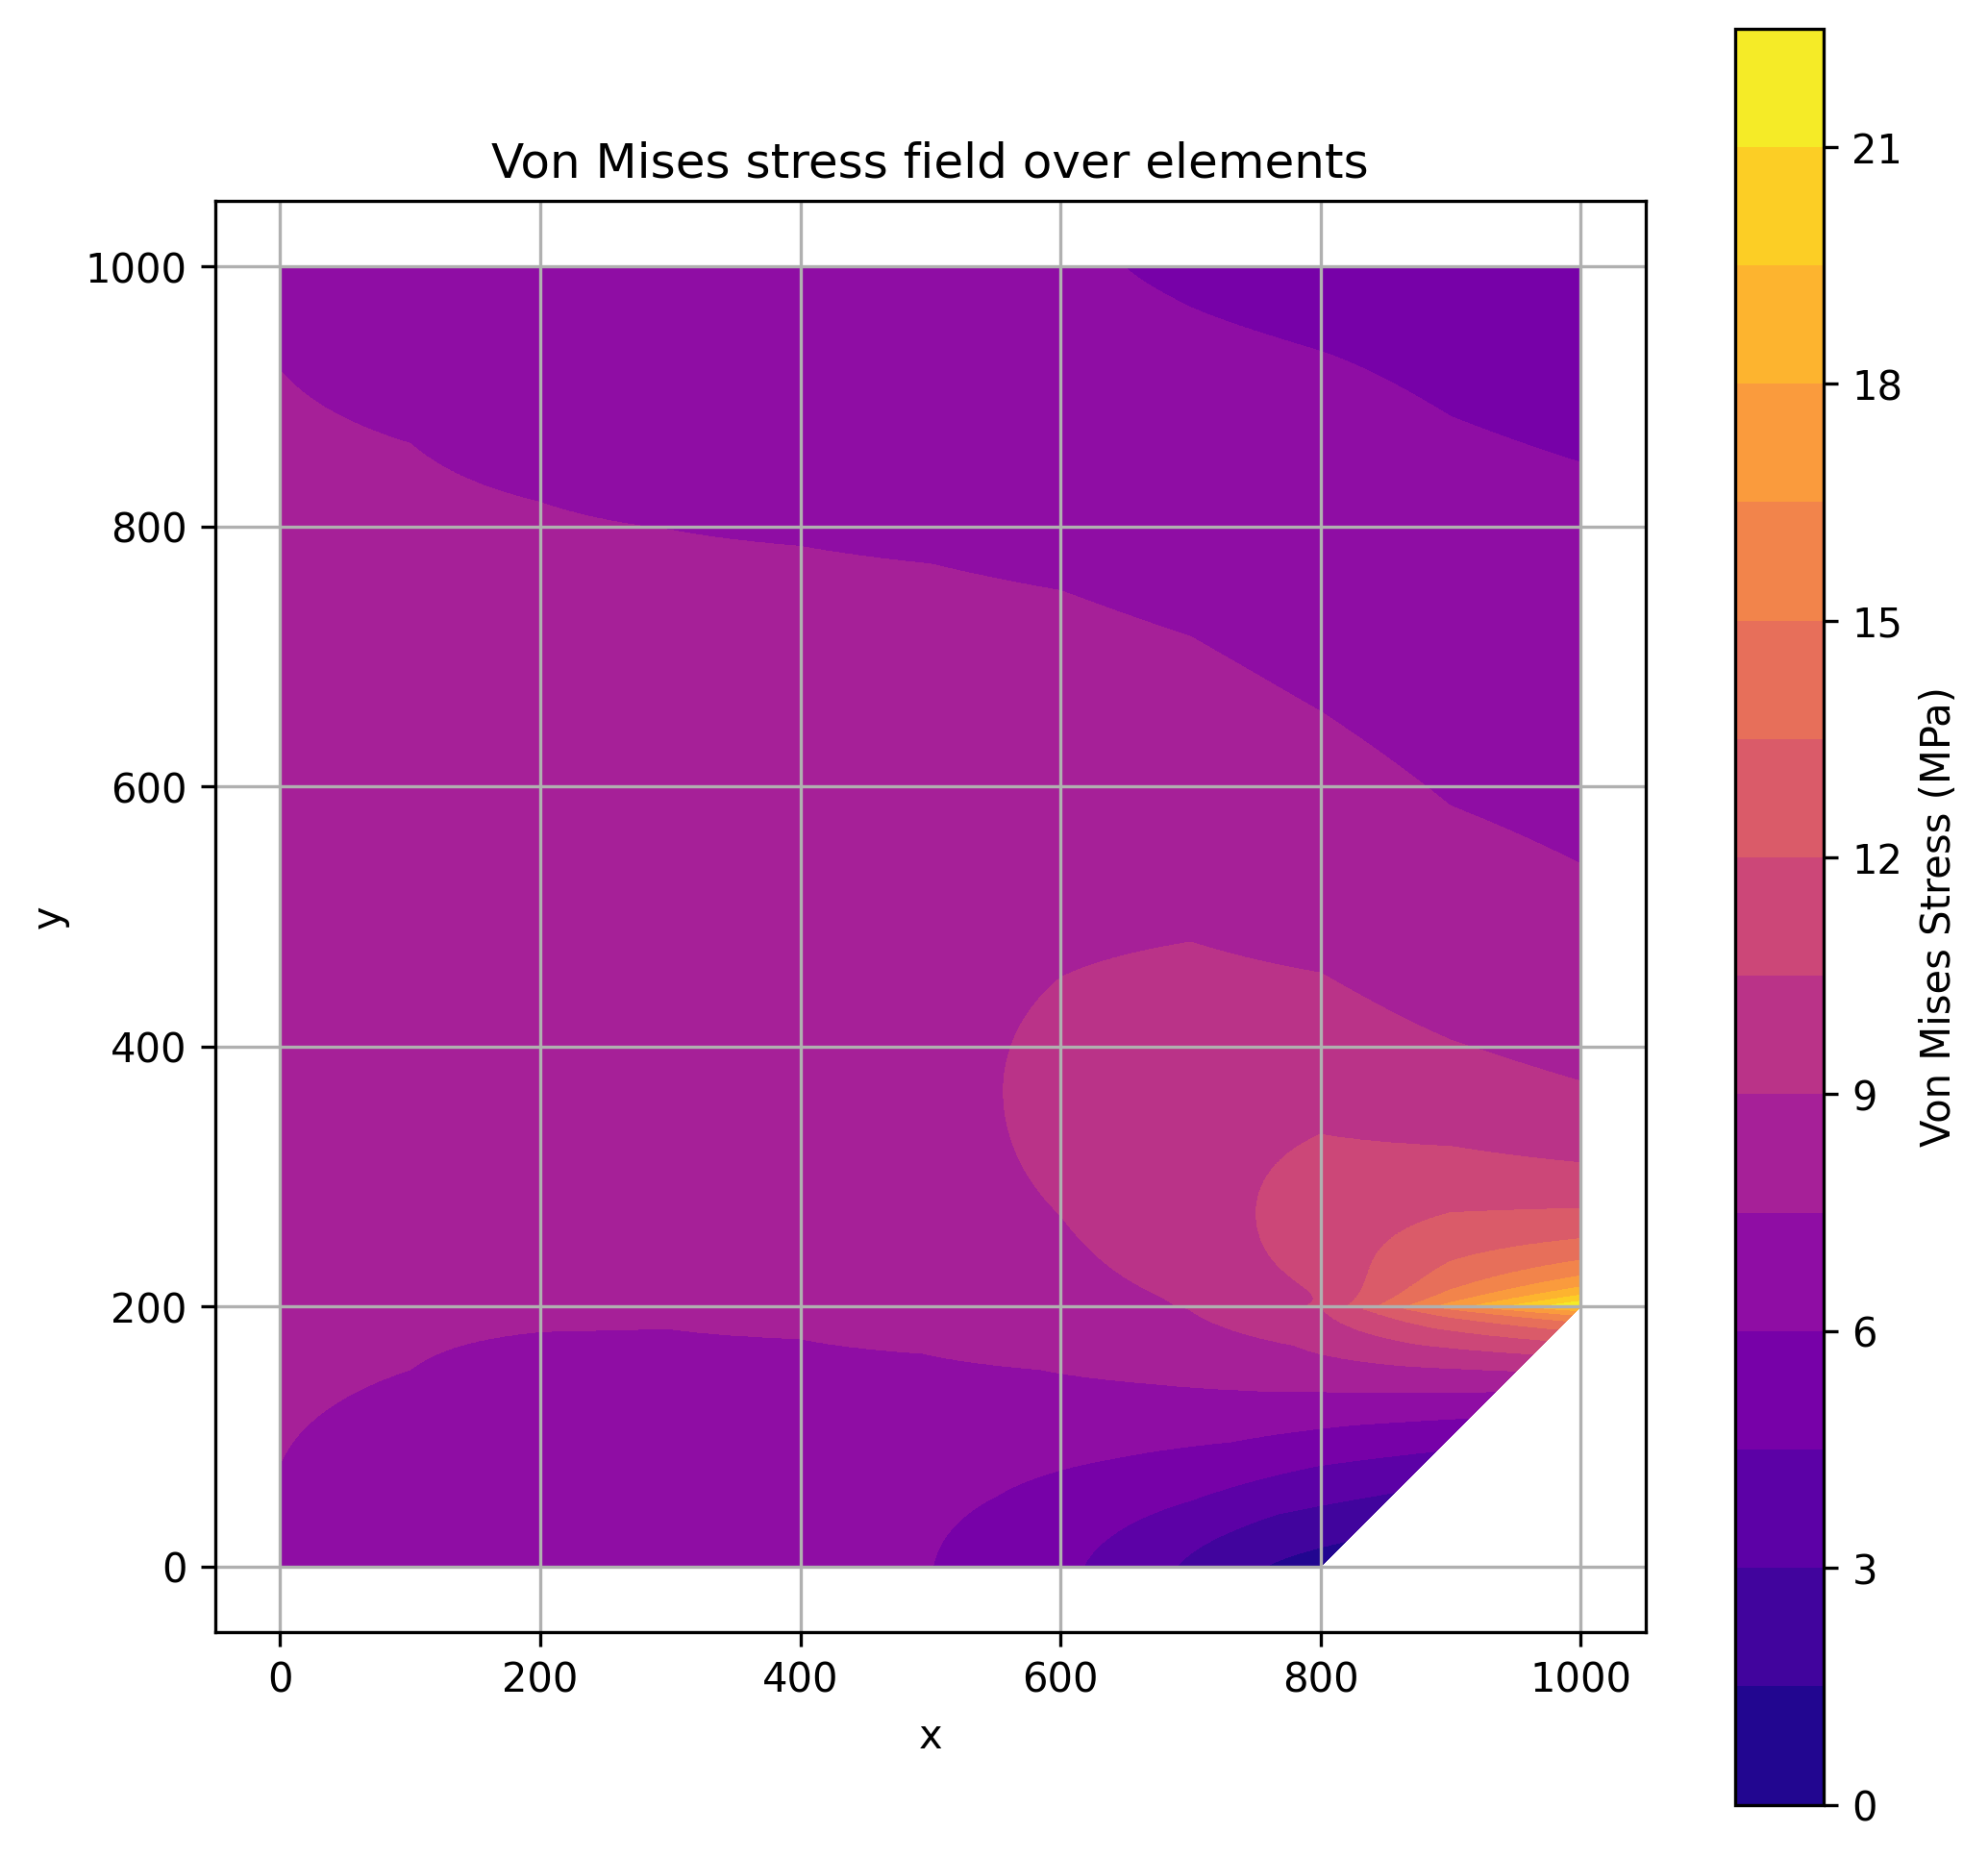
\includegraphics[width=\textwidth]{GRAFICOS/Quad9/1.25mm_global/resultados_von_mises.png}
    \caption{Global mesh refinement - $h=1.25mm$}
    \label{fig:img13}
  \end{subfigure}
  \hfill
  \begin{subfigure}[b]{0.45\textwidth}
    \centering
    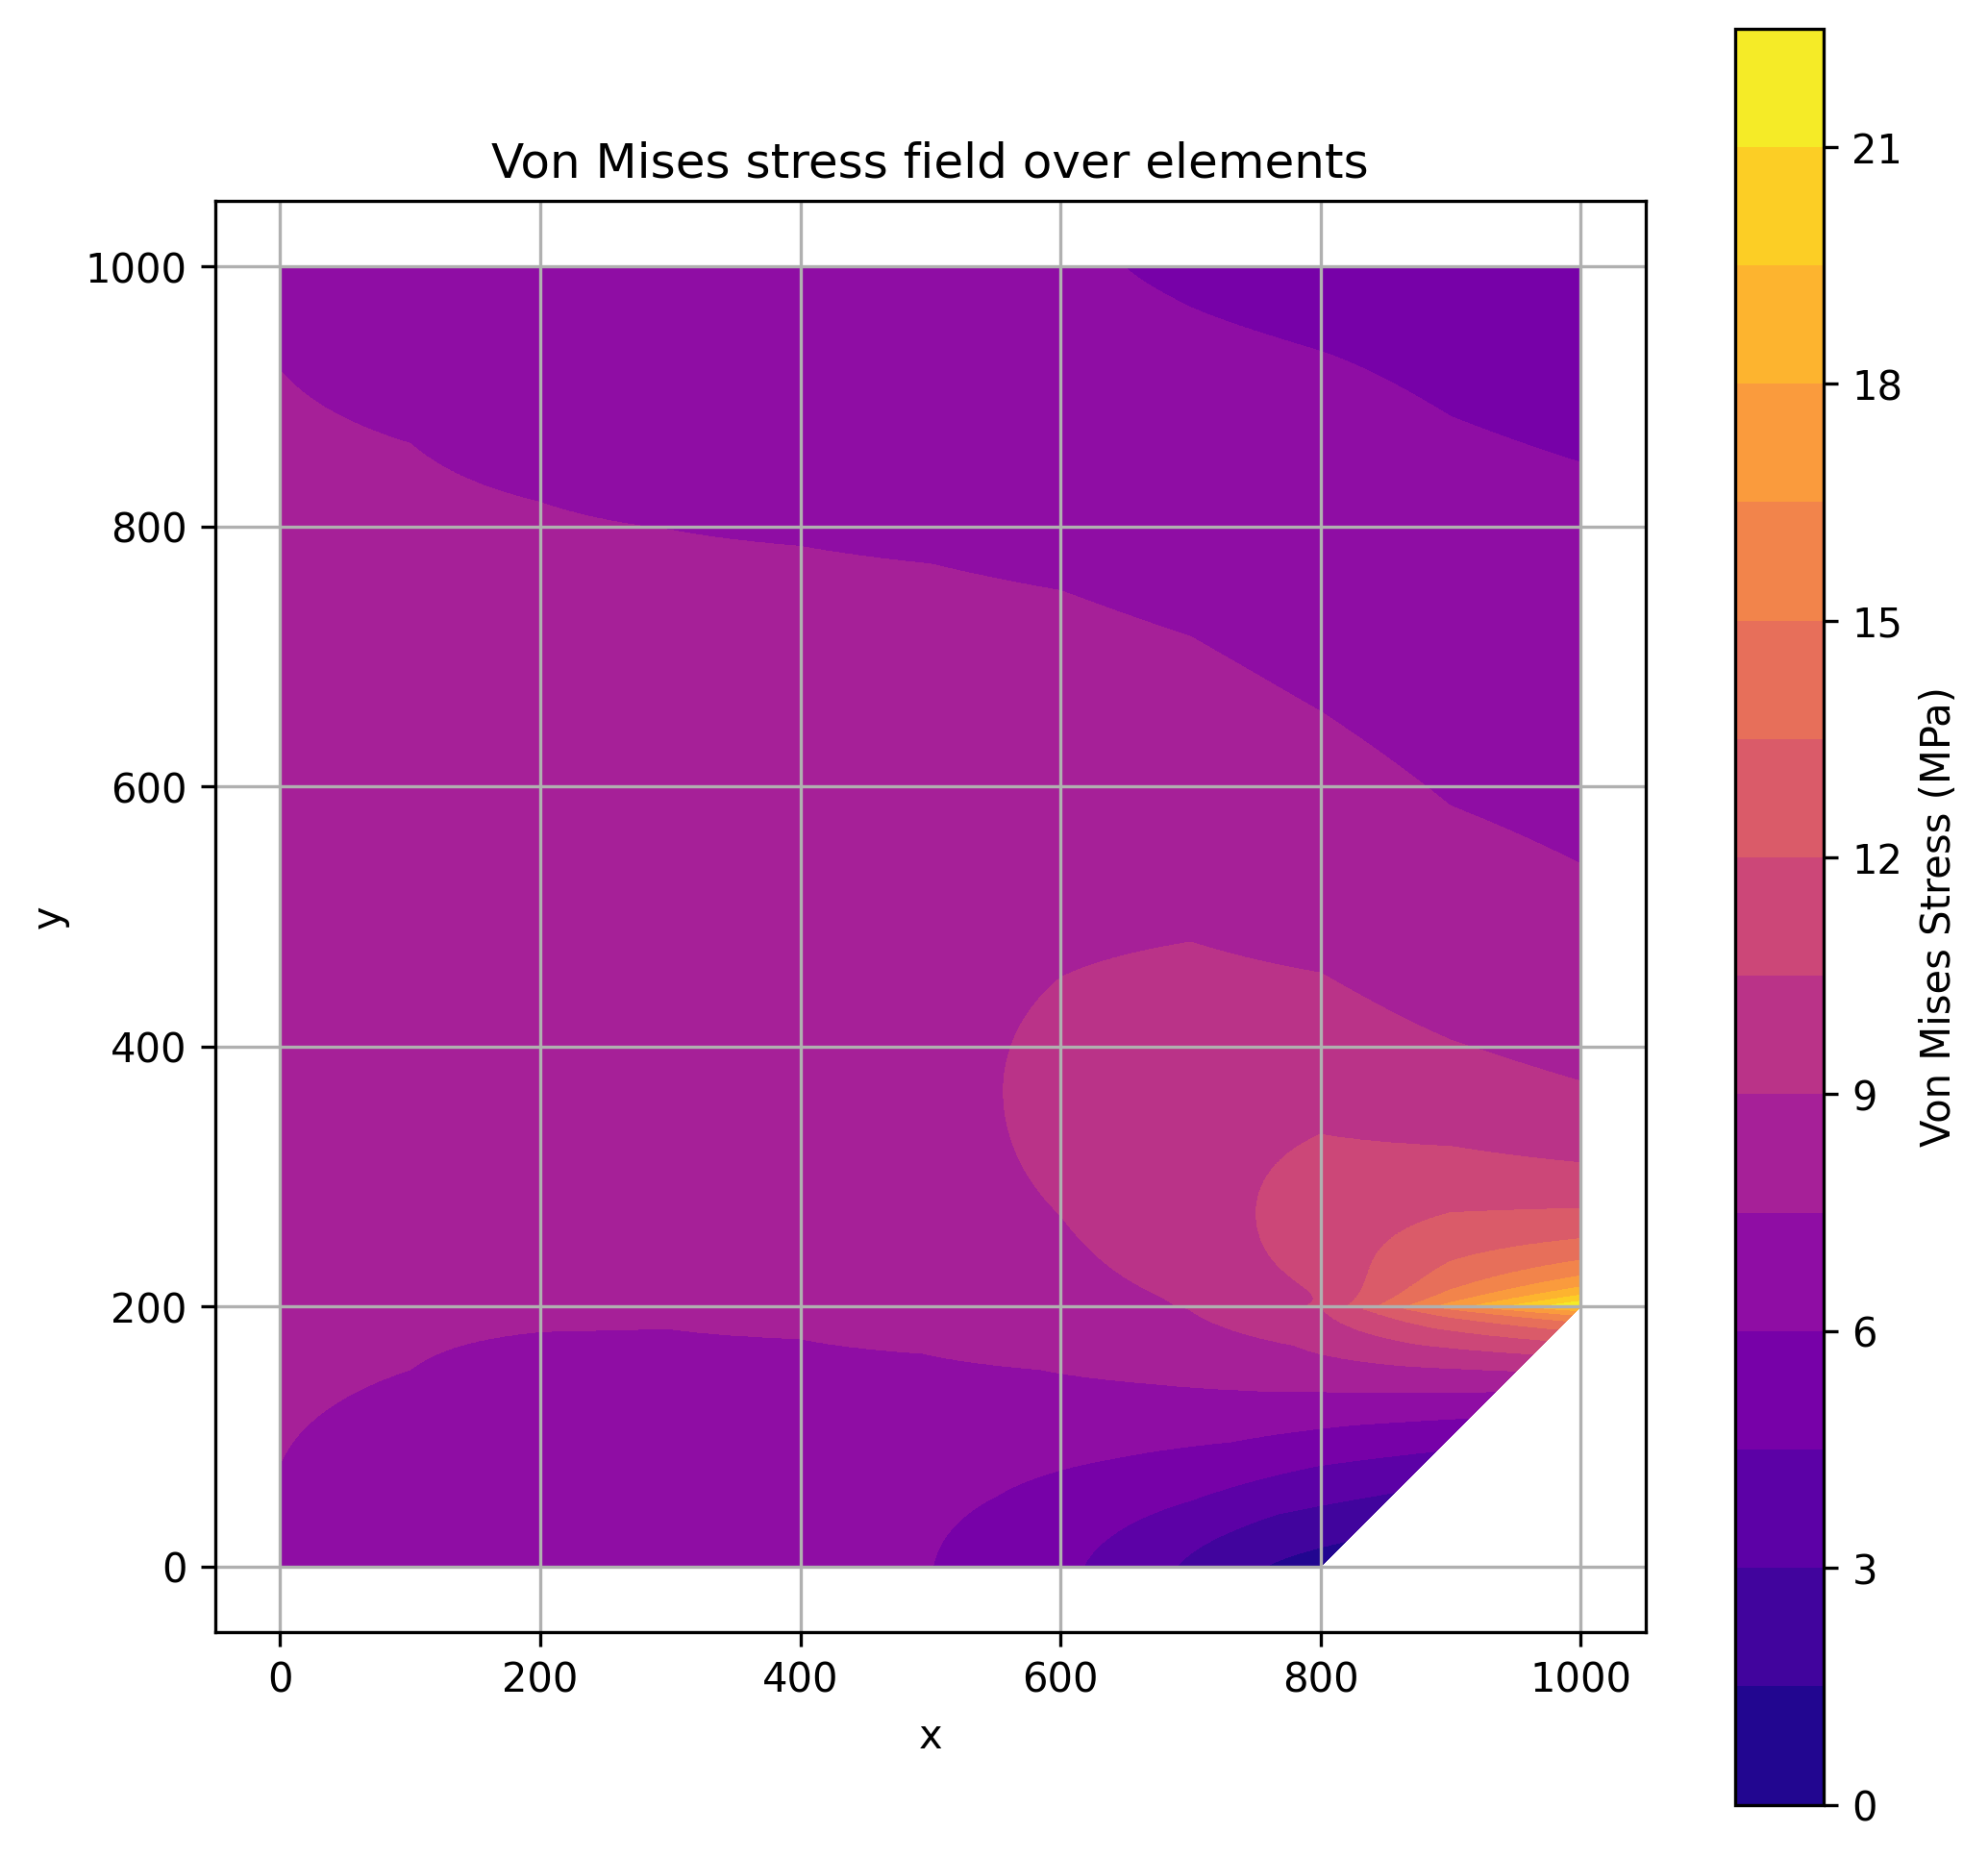
\includegraphics[width=\textwidth]{GRAFICOS/Quad9/1.25mm_global/resultados_von_mises.png}
    \caption{Local mesh refinement - $h=1.25mm$}
    \label{fig:img23}
  \end{subfigure}
\end{figure}

\subsection{Part c)}

In this section, an optimization of the strcutre was made. Moreover, it was modeled and simulated, reulting in a complete stress and behaviour analysis.

The main objective was to anulate the stress concentration sections, in order to reduce the maximum stress in the strcuture and compare it with the previous results.






\end{document}